\documentclass[11pt]{article}

\title{\color{navyblue} Difference-in-Differences Estimation with Spatial Spillovers\thanks{I am grateful to Taylor Jaworski, Adam McCloskey, Damian Clarke, Daniel Kaffine, Tania Barham, Alexander Bentz, James Flynn, Brach Champion, Hannah Denker, and participants of the CU Boulder Labor Economics Seminar for helpful comments.}}
\author{\normalsize Kyle Butts\\{\footnotesize Univ. of Colorado, Boulder}}
\date{\footnotesize\today}

% Margins ----------------------------------------------------------------------

\usepackage[margin=1.25in]{geometry}

% AMS --------------------------------------------------------------------------

\usepackage{amsmath}
\usepackage{amsfonts}
\usepackage{amsthm}
\usepackage{graphicx}


% Line Spacing -----------------------------------------------------------------

\renewcommand{\baselinestretch}{1.5}


% Font -------------------------------------------------------------------------

\usepackage[T1]{fontenc}
\usepackage[default]{lato} % Lato as text font
% \usepackage[utopia, varg]{newtxmath}
% \renewcommand{\rmdefault}{futs} % Utopia as text font 

% Small adjustments to text kerning
\usepackage{microtype}

% Remove annoying over-full box warnings
\vfuzz2pt 
\hfuzz2pt


% Tikz support -----------------------------------------------------------------

\usepackage{tikz}


% Color Palette ----------------------------------------------------------------

\usepackage{xcolor}

% https://www.materialpalette.com/colors
\definecolor{dark-maroon}{HTML}{5D0F0D}
\definecolor{navyblue}{HTML}{0A3044}

% From Davidson Mackinnon
\definecolor{dm-blue}{HTML}{086fbd}
\definecolor{dm-red}{HTML}{ba3132}
\definecolor{dm-green}{HTML}{3f7e32}

% https://www.viget.com/articles/color-contrast/
\definecolor{purple}{HTML}{5601A4}
\definecolor{navy}{HTML}{0D3D56}
\definecolor{ruby}{HTML}{9a2515}
\definecolor{alice}{HTML}{107895}
\definecolor{daisy}{HTML}{EBC944}
\definecolor{coral}{HTML}{F26D21}
\definecolor{kelly}{HTML}{829356}
\definecolor{cranberry}{HTML}{E64173}
\definecolor{jet}{HTML}{131516}
\definecolor{asher}{HTML}{555F61}
\definecolor{slate}{HTML}{314F4F}


% Hyperlinks -------------------------------------------------------------------

\usepackage{hyperref}
\hypersetup{
    colorlinks= true,
    citecolor= dark-maroon,
    linkcolor= dark-maroon,
    filecolor= dark-maroon,      
    urlcolor= dark-maroon,
}


% Citations --------------------------------------------------------------------

% note, natbib provides better hyperlinking
\usepackage{natbib}
\bibliographystyle{econ-aea}


% Define Theorems --------------------------------------------------------------

% Put proper spacing after Theorem #. 
\newtheoremstyle{spacing}
{}%          Space above, empty = `usual value'
{}%          Space below
{}%  Body font
{}%          Indent amount (empty = no indent, \parindent = para indent)
{\bfseries\color{navyblue}}% Thm head font
{.}%         Punctuation after thm head
{2.5mm}%  Space after thm head: \newline = linebreak
{}%          Thm head spec

% note, theorem is the name that goes in \begin{} and Theorem is the name displayed as Theorem 1
\theoremstyle{spacing}
\newtheorem{theorem}{Theorem}
\newtheorem{proposition}{Proposition}
\newtheorem{assumption}{Assumption}
\newtheorem{example}{Example}


% Custom Math Definitions ------------------------------------------------------

\newcommand{\expec}[1]{\mathbb{E}\left[#1\right]}%
\newcommand{\condexpec}[2]{\mathbb{E}\left[#1 \ \vert \ #2\right]}%
\newcommand{\prob}[1]{\mathbb{P}\left[#1\right]}%
\newcommand{\var}[1]{\mathrm{Var}\left[#1\right]}%
\newcommand{\cov}[1]{\mathrm{Cov}\left[#1\right]}%
\newcommand{\one}{\mathbf{1}}


% Titlepage --------------------------------------------------------------------

% \maketitle
\usepackage{titling}
\usepackage{setspace}

% title
\pretitle{\begin{spacing}{1}\begin{flushleft}\huge}
\posttitle{\end{flushleft}\end{spacing}\vspace{-5mm}}
% author, note don't use \and 
\preauthor{\begin{flushleft}\LARGE}
\postauthor{\end{flushleft}\vspace{-7.5mm}}
% date
\predate{\begin{flushleft}\Large\color{asher}}
\postdate{\end{flushleft}\vspace{-5mm}}

% Abstract
\renewenvironment{abstract}
 {\noindent\rule{\linewidth}{.5pt}\noindent}
 {\noindent\rule{\linewidth}{.5pt}}

% alternative abstract
% \renewenvironment{abstract}
% {
%   \centerline {\large \bfseries \scshape \color{navyblue} Abstract}
%   \begin{quote}
% }
% {\end{quote}}


% Section and Subsection Styling -----------------------------------------------

\usepackage[explicit]{titlesec}

\titleformat{\section}
  {\Large \bf \color{navyblue}}
  {\thesection \,---}
  {0.25em}
  {#1}
  
\titleformat{\subsection}
  {\fontsize{11}{10}\it}
  {\thesubsection.}
  {1em}
  {#1}

% Don't number subsubsection
\setcounter{secnumdepth}{2}

% Footnote ---------------------------------------------------------------------

% Spacing between footnotes on same page
\addtolength{\footnotesep}{1mm}

% Space after footnote number
\let\oldfootnote\footnote
\renewcommand\footnote[1]{\oldfootnote{\ #1}}

% No footnote line
\renewcommand\footnoterule{}

% No supsercript in footer
\makeatletter
\renewcommand\@makefntext[1]{%
    \parindent 1em \noindent
    \hb@xt@1.8em{\hss\normalfont\@thefnmark.\hfill}#1
  }
\makeatother




% Enumerate/Itemize ------------------------------------------------------------

\usepackage{enumitem}
\setitemize{labelindent=0.5em,labelsep=0.25cm,leftmargin=*}
\setenumerate{labelindent=0.5em,labelsep=0.25cm,leftmargin=*}


% Table and Figure labelling ---------------------------------------------------

\usepackage{caption}

\DeclareCaptionLabelSeparator{threedash}{\,---\,}
\DeclareCaptionFont{navyblue}{\color{navyblue}}
\DeclareCaptionFont{jet}{\color{jet}}
\captionsetup[table]{format=plain, labelsep=threedash, font={navyblue, bf}}
\captionsetup[figure]{format=plain, labelsep=threedash, font={navyblue, bf}}

% Alternative: Left align captions
% \captionsetup[table]{labelfont=it, textfont={navyblue, bf}, labelsep=newline, justification=raggedright, singlelinecheck=off}
% \captionsetup[figure]{labelfont=it, textfont={navyblue, bf}, labelsep=newline, justification=raggedright, singlelinecheck=off}

% multifigure with \caption
% \begin{subfigure}\caption{} \end{subfigure}
\usepackage{subcaption}
\captionsetup[subfigure]{format=plain, font={jet, footnotesize, bf}}


% Tables -----------------------------------------------------------------------

% Fix \input with tables
% \input fails when \\ is at end of external .tex file

\makeatletter
\let\input\@@input
\makeatother

% Make tables/figures wider than \textwidth using:
% \begin{adjustbox}{width = 1.2\textwidth, center}
% \end{adjustbox}
\usepackage{adjustbox}

% Slighty more spacing between rows
\usepackage{array}
\renewcommand\arraystretch{1.2}

% Table with easy to use footnotes
% \begin{threeparttable}
%    \begin{tabular} ... \end{tabular}
%    \begin{tablenotes}
%        \item \textit{Notes.}
%    \end{tablenotes}  
% \end{threeparttable}
\usepackage[flushleft]{threeparttable}
\setlength\labelsep{0pt}

% \toprule, \cmidrule, \bottomrule
\usepackage{booktabs}

% If tables are too narrow, fill columns using:
% \begin{tabularx}{\linewidth}{cols}
% col-types: X - center, L - left, R -right
% If you want relative scale for columns: 
% >{\hsize=.8\hsize}X/L/R
\usepackage{tabularx}
\newcolumntype{L}{>{\raggedright\arraybackslash}X}
\newcolumntype{R}{>{\raggedleft\arraybackslash}X}
\newcolumntype{C}{>{\centering\arraybackslash}X}

% Shorter multicolumn commands
\newcommand{\mcc}[1]{\multicolumn{1}{c@{}}{#1}}
\newcommand{\mcl}[1]{\multicolumn{1}{l@{}}{#1}}
\newcommand{\mcr}[1]{\multicolumn{1}{r@{}}{#1}}

% d column
\usepackage{dcolumn}
\newcolumntype{d}[1]{D..{#1}}

% Landscape table 
% \begin{landscape} \pagestyle{lscaped} table... \end{landscsape}
% \usepackage{pdflscape} - rotates page left-side up in pdf
% \usepackage{lscape} - does not rotate page, only figure/table

\usepackage{pdflscape}

% For landscape, fix page number location
\usepackage{fancyhdr}
\fancypagestyle{lscaped}{%
    \fancyhf{}
    \renewcommand{\headrulewidth}{0pt}
    \textnormal
    \fancyfoot{%
        \tikz[remember picture,overlay]
        \node[outer sep=2.5cm,above,rotate=90] at (current page.east) {\thepage};
    }
}
  

% ------------------------------------------------------------------------------

%\addbibresource{references.bib}
\hypersetup{pdftitle={Difference-in-Differences Estimation with Spatial Spillovers}, pdfauthor={Kyle Butts}}

\begin{document}

% ------------------------------------------------------------------------------
\begin{titlepage}
    \maketitle
    
    \begin{abstract}
        Empirical work often uses treatment assigned following geographic boundaries. When the effects of treatment cross over borders, classical difference-in-differences estimation produces biased estimates for the average treatment effect. In this paper, I introduce a potential outcomes framework to model spillover effects and decompose the estimate's bias in two parts: (1) the control group no longer identifies the counterfactual trend because their outcomes are affected by treatment and (2) changes in treated units' outcomes reflect the effect of their own treatment status and the effect from the treatment status of ``close'' units. I propose estimation strategies that can remove both sources of bias and semi-parametrically estimate the spillover effects themselves. I extend \citet{Callaway_SantAnna_2020} to allow for event-study estimates that control for spillovers. To highlight the importance of spillover effects, I revisit analyses of three place-based interventions. 
    \end{abstract}
\end{titlepage}
% ------------------------------------------------------------------------------



% ------------------------------------------------------------------------------
\section{Introduction}
% ------------------------------------------------------------------------------

Empirical work often considers settings where policy is targeted to groups of units by geographic boundaries, but the effect of these treatments spillover onto `nearby' units.\footnote{The framework of this paper applies to any setting with a well-defined measures of distance, e.g. geographic distance, economic distance such as supply chains, node distance in a graph, or social relationships in schools or cities.} Place-based policies, programs that are targeted to specific locations, are known to have general-equilibrium effects that extend far past the area intended to receive treatment \citep{Kline_Moretti_2014b}. Spillover effects can occur on to both control and treated units. First, there can be spillover effects onto control units. For example, individuals in control areas can travel to the treated areas and receive treatment (e.g. a hospital opening serves nearby residents) or changes in the economy in a treated area can have feedback loops that affect nearby economies (e.g. a new factory opening increases service sector spending). Second, there can be spillover effects onto other treated units. For example, forces of agglomeration can increase effects as treatment concentration increases (e.g. knowledge-sharing between workers), forces of congestion or market competition can decrease the effects of treatment (e.g. bidding up of wages cause employment effects of factory openings to be mitigated), and treatment effectiveness may be improved by multiple jurisidictions learning from one another. 

In this paper, I introduce a potential outcome framework that directly models spillover effects. Using this framework, the central theoretical result of my paper is that in the presence of spillovers, the standard difference-in-differences estimate identifies the direct effect of treatment (the estimand of interest) plus two additional bias terms resulting from the spillovers.\footnote{The term `direct' effect can refer to either the average treatment effect on the treated or the intent to treat effect. In empirical applications, the `direct` effect is sometimes called the `partial equilibrium' effect or the `local' effect.} The intuition for why the two forms of spillovers cause bias is as follows. 

First, untreated units that are `close' to treated units experience effects of treatment and therefore these `control' units fail to identify the counterfactual trend. When estimating by difference-in-differences, the spillover onto the `close' control units is averaged into the untreated units' change in outcomes. In this case, the spillover is subtracted from the estimated treatment effect and biases the estimate in the opposite sign of the spillover effect. 

For example, consider trying to estimate employment effects of a factory opening in a county. Agglomeration economies suggest that neighboring counties would also benefit from knowledge spillovers and improved access to supply chain which would potentially increase economic activity \citep{Duranton_Puga_2003}. The treatment effect estimate is negatively biased because the change in outcome in neighboring counties is higher than it would be absent treatment. Researchers would therefore underestimate the positive benefits of treatment.\footnote{If the policy maker had a welfare function that included both treated and neighboring counties, they would fail to count the positive benefits of the control units and they would underestimate the positive benefits on the treated units. Difference-in-differences estimation would therefore result in double undercounting.}

% Despite the problem of spillovers being common across many settings, \citet{Berg_Streitz_2019} document that little empirical analysis directly controls for spillovers when estimating the `direct' effect of treatment on the treated units.

Second, changes in treated units' outcomes reflect the effect of their own treatment status and the effect from the treatment status of ``close'' units.The spillover onto other treated units is averaged into the treated units' change in outcomes. Therefore the bias of treatment effect is the same sign as the sign of the spillover. Continuing with our example, two factory openings in neighboring counties might cause the benefit of each individual factory to increase due to agglomeration forces. The estimated treatment effect will count the `direct' effect of the factory opening as well as the benefit of the agglomeration economies from nearby factory openings. Therefore the treatment effect will be positively biased due to the positive spillover onto also treated units.

I then use my potential outcome framework to evaluate commonly used empirical strategies found in applied work and provide practical recommendations for researchers. The most common approach is to remove potentially contaminated control units from the sample in order to remove spillover effects on control units \citep{Berg_Streitz_2019}. This approach is not recommended for two reasons. First, the removal of too few control units will leave bias and removal of too many will lower precision of the treatment effect estimate. This results in a bias-variance trade-off that other approaches do not share. Second, this method does not remove spillover effects on treated units and will leave this bias term in the difference-in-differences estimate. Another common approach is to include either an indicator or a set of rings around treated units. This approach will remove all bias from the spillover effects on control units provided that all control units with spillover effects are included in the indicator. Similar to the previous approach, spillover effects on also treated units still add bias to estimates of the direct effect.

Therefore, I propose an estimation strategy that will remove both sources of bias with very minimal assumptions on the structure of spillovers. To remove \textit{all bias} from the direct effect estimate, a researcher needs to just include an indicator for being close to a treated unit interacted with treatment status, so long as the indicator captures all units affected by spillovers. In my decomposition of the treatment effect estimate, the bias terms are the \textit{average} spillover effects onto treated and control units. An indicator variable interacted with treatment status therefore can estimate these two averages and remove them from the difference-in-differences estimate. Importantly, my method does not require researchers to make any assumptions about how spillover effects propagate across space. The only assumption required is the maximum distance from treated units spillovers can occur.\footnote{Even if the maximum distance is not large enough, since treatment effects typically decay over distance, most of the bias will still be removed. Including too many units in the indicator will increase the variance in the estimates for average spillover effects as the other control units identify the parallel counterfactual unit.} 

Since spillover effects are often important causal effects themselves, I next turn to how to estimate spillovers directly. I show with evidence from Monte Carlo simulations, that commonly used semi-parametric estimation strategies capture spillovers well (in a mean square prediction error sense). This involves creating a set of distance bins from treated units (e.g. being 0-20 miles, 20-40 miles, 40-60 miles from treated unit) and interacting them with a treatment indicator.\footnote{The choice of the distance bins depends on the economic context and in particular the source of the spillovers.} The key consideration required by a researcher is whether the size of spillover effects are additive in the number of nearby treated units or not. For non-additive spillovers, I recommend a set of mutually-exclusive indicators which measures which distance bin that the \textit{closest} treated unit falls within for a given observation. For additive spillovers, I recommend using the \textit{number of} treated units within each distance bin for a given observation.\footnote{While the non-additive version of ring indicators will remove all bias from the direct effect of treatment even under misspecification, this is not true of additive rings. Therefore, researchers may want to estimate the direct effect of treatment using non-additive rings and then use additive rings to estimate spillover effects.} 

To show the importance of considering spillover effects, I revisit analyses of place-based policies in urban economics in Section \ref{sec:tva}. I revisit the analysis of the Tennessee Valley Authority by \citet{Kline_Moretti_2014}. The Tennessee Valley Authority was a large scale New Deal program that created many new dams for flood-protection and navigation. The construction of large-scale dams lowered the cost of power for industrial firms giving the region an industrial boost \citep{Kitchens_2014}. The scale of federal investment in the region was large and the pro-manufacturing benefits likely spread further than the Authority's boundary due to the electrification infrastucture and agglomeration economies \citep{Severnini_2014}. I show that estimation by difference-in-differences fails to account for these spillovers and therefore forms biased estimates of the local effect of the Tennessee Valley Authority.

Following this empirical application, I discuss how my framework fits into a larger discussion on identification strategies with place-based policies. I revisit conflicting results about United States' federal Empowerment Zones, a program that creates incentives for businesses to locate in high-poverty neighborhoods. \citet{Busso_Gregory_Kline_2013} use Census Tracts from qualified but ultimately rejected applications that are typically far away from accepted Zones as a comparison group and find that significant reductions in poverty. This empirical strategy is based on the idea that since they also qualified for the program, these comparison units would be on parallel trends without being contaminated by spillover effects from treatment. \citet{Neumark_Kolko_2010}, on the other hand, use census tracts within 1,000 feet of the Zone and find no statistically significant effects. This empirical strategy assumes that the borders are drawn somewhat randomly and therefore being just outside is as good as random. Although, using close units is potentially problematic as they can experience spillover effects from the Zones. My framework can explain the differences in findings if there are positive spillover effects onto census tracts just outside Empowerment Zones. 

Last, in Section \ref{sec:event_study}, I extend estimation of the direct effect and spillover effects of treatment into the event study framework by extending the work of \citet{Callaway_SantAnna_2020}. This allows for a very common setting in which treatment turns on for different units in different periods. I first show how to adjust their methods to control for spatial spillovers in estimation of treatment effects. Then, I show how to estimate average spillover effects. My paper is the first paper to study estimation of treatment effects in an event-study framework in the presence of spillover effects. 

I demonstrate the method by revisiting the analysis by \citet{Bailey_Goodman_Bacon_2015} of Community Health Centers which provided low-cost primary care to impoverished areas. They find that the health centers significantly lowered the mortality rate in treated counties. I find that in this context, since the mortality declines caused by the health centers was due to primary care, spillover effects are near-zero. This result shows the importance of accessability concerns when deciding the location of the health centers.

% ------------------------------------------------------------------------------
\subsection{Relation to the Literature} 
% ------------------------------------------------------------------------------

There is a large literature on estimation of treatment effects in the presence of spillovers using a `partial identification' framework where units are in distinct treatment clusters and outcomes depend on the treatment status within the observation's cluster only.\footnote{ \citet{Angelucci_DiMaro_2016} provides an overview of estimation of treatment effects in the presence of ``within-group'' spillovers. Examples in the literature include: \citet{Halloran_Struchiner_1995} consider community-vaccine rates in epidemology; \citet{Miguel_Kremer_2004} consider deworming programs in Kenyan schools; \citet{Sobel_2006} considers interference in the Moving to Opportunity Program; and \citet{Angrist_2014} studies the context of school peer effects.} Estimation compares units in the partially treated clusters with control units in completely untreated clusters which do not receive spillover effects. This allows standard difference-in-differences estimation of both the direct effect (treatment effect on the treated) and spillover effects (treatment effect on the untreated in the treated clusters). 

There is a nascent literature exploring estimation of direct and spillover effects which does not require a completely untreated cluster by using a potential outcomes framework. \citet{Vazquez-Bare_2019} presents a potential outcomes model that explicitly accounts for ``within-group'' spillovers in experiments which allows for seperate estimation of direct effect and spillover effects by a simple differences-in-means. I extend this work by focusing on difference-in-differences estimation in non-experimental settings.  \citet{Savje_Aronow_Hudgens_2019} consider estimation of treatment effects by difference-in-differences, but they define treatment effects as the combination of direct effects and spillover effects. My paper develops a strategy to allow researchers to seperately identify treatment effects and spillovers. These estimates can be combined to estimate their definition of average treatment effect. The further advantage is that `net' treatment effects can be estimated at different levels of exposure which is more relevant for future policy decisions.

I also contribute to the literature that focuses on estimation of treatment effects with spatial spillovers using the difference-in-differences framework \citep{Clarke_2017,Berg_Streitz_2019,Verbitsky-Savitz_Raudenbush_2012,Delgado_Florax_2015}. I contribute to this literature in two ways. First, my paper derives an explicit form for this bias in terms of general potential outcomes which allows my results to capture many different forms of spillovers. For the above papers, if I assume the particular functional forms for potential outcomes, I arrive at the same bias equation as theirs if they have one derived explicitly. Second, my paper also advances the literature by considering estimation of direct effects and spillover effects in event-study framework which allows for the common occurence of staggered treatment adoption.

The rest of the paper is structured as follows. Section \ref{sec:po_framework} presents the potential outcomes framework, defines the estimand of interest, and shows the resulting bias from estimating a classical difference-in-differences model. Section \ref{sec:estimation} focuses on estimation of the direct and spillover effects of treatment. I evaluate currently used solutions in the literature and present a set of recommendations to more robust estimation strategies. Section \ref{sec:tva} presents an application for evaluating the Tennessee Valley Authority program. Section \ref{sec:event_study} discusses briefly how to incorporate spillovers into event-study estimation following the insights from \citet{Callaway_SantAnna_2020}. I apply these methods in evaluating spillover effects of U.S. Community Health Centers in Section \ref{sec:chc}.


% ------------------------------------------------------------------------------
\section{Potential Outcomes Framework}
\label{sec:po_framework}
% ------------------------------------------------------------------------------

This section will present a potential outcome framework that formalizes spatial spillovers. Following the canonical difference-in-differences framework, there are T periods and treatment turns on for all treated units at some period $t_0$ and remain on afterwards.\footnote{This framework is extended to staggered treatment adoption in Section \ref{sec:event_study}.} Potential outcomes, denoted $Y_{i,t}(D_i, h(\vec{D},i))$, for unit $i$ at time $t$ are a function of own treatment-status $D_i$ and, departing from the standard potential outcomes framework, of a function of the entire vector of treatment assignments $h(\vec{D}, i)$ where $\vec{D} \in \{0,1 \}^n$ denotes the $n$-dimensional vector of all unit treatments. The function $h(\vec{D}, i)$ is referred to as an `exposure mapping' and is a non-negative scalar- or vector- valued function. The exposure mapping measures the intensity at which unit $i$ is affected by spatial spillovers. When unit $i$ is sufficiently `far' away, it has no exposure to spatial spillovers and $h(\vec{D}, i) = \vec{0}$. The exposure mapping formalizes the SUTVA violation by summarizing how outcomes are affected by other unit's treatment assignment. To help better understand the exposure mapping function, I give three examples that are commonly used in the literature.

\begin{example}
    First, $h(\vec{D}, i)$ can be an indicator variable that equals one only if there is a treated unit within $\bar{d}$ miles of unit $i$.\footnote{Similarly a dummy for counties that share contiguous borders is commonly used.} Let $d(i,j)$ be a distance measure which tells the distance unit $i$ is from unit $j$.  In this case \begin{equation}\label{eq:h_within}
        h(\vec{D}, i) = \max_{i \neq j} D_j * \one[ d(i,j) < \bar{d} ] 
    \end{equation}
    This exposure mapping is a realistic specification when it is assumed that spillover effects do not decay over distance until $\bar{d}$ and the intensity of spillovers does not depend on the number of neighboring units treated. For example, this exposure mapping likely applies in the context of new library creation \citep{Berkes_Nencka_2020}. In this case the distance $\bar{d}$ would be the maximum distance people would travel to a nearby library. The benefits of access to a neighboring town library does not depend on whether people can access 1 or more nearby libraries, so the binary exposure mapping is a good approximation to spillovers in this context.  
\end{example}
    
\begin{example}
    Second, $h(\vec{D}, i)$ can be a function that equals the number of units treated within distance $\bar{d}$, i.e. \begin{equation}\label{eq:h_within_additive}
        h(\vec{D}, i) = \sum_{j} D_j * \one[ d(i,j) < \bar{d} ].
    \end{equation}
    This exposure mapping is no longer binary, so the intensity of spillovers is additive in the number of nearby units treated. In the context of large store openings, this exposure mapping captures the additive nature of agglomeration economies. As more nearby counties receive new stores, the force of agglomeration and therefore the spillover effect increases (e.g. \citet{Basker_2005}).
\end{example}
    
\begin{example}
    Last, $h(\vec{D}, i)$ is a spatial decay function where exposure decreases with distance. In this case, spillover intensity is the sum across all treated observations' decay term, i.e. \begin{equation}\label{eq:h_decay}
        h(\vec{D}, i) = \sum_{j \neq i} D_j e^{-\alpha d(i,j)}.
    \end{equation} 
    This exposure mapping allows for the intensity of spillovers to depend on distance to treatment and also is additive in the number of nearby units treated.\footnote{However, this specification assumes that all units are affected by all other units. This creates problems with inference because it implies potential correlation between all units' error terms. For this reason, this function often is summed over only the $k$-nearest neighbors or over units within $\bar{d}$ miles.} The speed that spillover effects decay over distance depends on the parameter $\alpha$ that can be calibrated by the researcher or estimated using a non-linear least squares routine. In the literature on R\&D investment, for example, \citet{Keller_2002} uses a modified version of this exposure mapping where $D_j$ is country $j$'s R\&D expenditure. This specification features exponential decay over distance which captures the theoretical insight that research spending in closer locations has a larger effect than further away spending.
\end{example}

After chosing an exposure mapping that makes sense in the economic context, a researcher must also specify the functional form of the potential outcomes. Typically, the exposure mapping enters into the regression linearly and potentially the coefficient is allowed to differ by treatment status to reflect that spillovers on control and treated units can be different phenomenon. 

% The results of this paper allows estimation and controlling for spillovers without needing to know the functional form of the exposure mapping. 
% TODO: Finish



% ------------------------------------------------------------------------------
\subsection{Spatial Spillovers}
% ------------------------------------------------------------------------------

With the potential outcomes defined, I define `spillover effects' as: \[
    Y_{i,t}(D_i, h(\vec{D}, i)) - Y_{i,t}(D_i, \vec{0}).
\] 
The spillover effect measures the difference in potential outcomes between being exposed at intensity $h(\vec{D}, i)$ and not being exposed. This effect can differ for either treated or control units as the magnitude or even the nature of spillovers might differ between treated and untreated units. Then, the average spillover effect onto control/treated units averages over potential heterogeneity in the effect size of spillovers and over heterogeneity in exposure intensity $h(\vec{D}, i)$: \[
    \tau_{\text{spill,control}} \equiv \expec{Y_{i,t}(D, h(\vec{D}, i)) - Y_{i,t}(D, \vec{0}) \ \vert \ D_i = D}.
\]
To emphasize, the average spillover effect onto conrol/treated units averages over each unit's exposure mapping which can be heterogeneous across units. For example, spillover effects can decay over distance as in Equation (\ref{eq:h_decay}) and the average spillover effect averages across different exposure intensities. 

It is important to clarify what I am assuming is the estimand of interest researchers would like to estimate when using difference-in-differences because there are multiple potential estimands defined in the literature. I assume that what the `average treatment effect' is trying to measure in this context is what I will call the `direct effect of treatment': \[
    \tau_{\text{direct}} = \expec{Y_{i,t}(1, \vec{0}) - Y_{i,t}(0, \vec{0}) \ \vert \ D_i = 1},
\] 
which measures the effect of being treated in the absence of exposure to spillovers. 

My definition of the direct effect of treatment differs from \citet{Savje_Aronow_Hudgens_2019} where they define the average treatment effect as \[ 
    \expec{Y_{i,t}(1, h(\vec{D}, i)) - Y_{i,t}(0, h(\vec{D}, i)) \ \vert \ D_i = 1},
\] 
where the expectation is over individuals and over different levels of exposures. The difference between their treatment effect and mine becomes more clear by adding and subtracting terms and rearranging:
\begin{align*}
    &Y_{i,t}(1, h(\vec{D}, i)) - Y_{i,t}(0, h(\vec{D}, i)) \\
    &\quad\quad = Y_{i,t}(1, h(\vec{D}, i)) - Y_{i,t}(1, 0) + Y_{i,t}(1, 0) - Y_{i,t}(0,0) + Y_{i,t}(0,0) - Y_{i,t}(0, h(\vec{D}, i)) \\
    &\quad\quad = \underbrace{Y_{i,t}(1, 0) - Y_{i,t}(0,0)}_{\text{Direct Effect}} + \underbrace{Y_{i,t}(1, h(\vec{D}, i)) - Y_{i,t}(1, 0)}_{\text{Spillover on Treated}} - \underbrace{(Y_{i,t}(0, h(\vec{D}, i)) - Y_{i,t}(0,0))}_{\text{Spillover on Control}} 
\end{align*}
The individual treatment effect \citet{Savje_Aronow_Hudgens_2019} use is the direct effect of treatment plus the difference between spillover on treated units and spillover on control units. 

I prefer my definition of the direct effect because it allows for seperate identification of the direct effect of treatment and the spillover effects themselves. The alternative estimand averages over exposure intensities and therefore is difficult to be used by a policy maker in a particular location. That is, a county deciding whether to implement a policy will want to consider the treatment effect plus the difference in spillover effects at \textit{a particular} exposure intensity. The estimand proposed by \citet{Savje_Aronow_Hudgens_2019} returns the average of spillovers across levels of exposure and can not be used to predict spillovers at specific exposure intensities while my preferred method of identifying the three effects seperately can. Estimates of the direct effect and spillover effect can be later combined to estimate the average treatment effect as defined by \citet{Savje_Aronow_Hudgens_2019}.




% ------------------------------------------------------------------------------
\subsection{Bias in Difference-in-Differences Estimation}
% ------------------------------------------------------------------------------

In this section, I identify the two sources of bias in difference-in-differences estimation of the direct effect of treatment. Researchers typically estimate the canonical two-way fixed effects model, 
\begin{equation}\label{eq:twfe}    
    y_{i,t} = \tau D_{i,t} + \mu_i + \mu_t + \epsilon_{i,t},
\end{equation}
where $D_{i,t} = D_i \one(t = 1)$. The estimator $\hat{\tau}$ is a biased estimate for $\tau_{\text{direct}}$ in the presence of spillovers. To show this, I first present the equivalent to the parallel counterfactual trends assumption in the context of the new potential outcome framework. 

\begin{assumption}[Parallel Counterfactual Trends]\label{assumption:parallel}
    \[ 
        \expec{\bar{Y}_{i,Post}(0, \vec{0}) - \bar{Y}_{i,Pre}(0, \vec{0}) \ \vert \ D_i = 1 } = 
        \expec{\bar{Y}_{i,Post}(0, \vec{0}) - \bar{Y}_{i,Pre}(0, \vec{0}) \ \vert \ D_i = 0 },
    \]
    where $\bar{Y}_{i,W}$ is the average outcome in either the post- or pre-periods.
\end{assumption}
This assumption states that in the absence of treatment and with zero exposure (not just the absence of individual $i$'s treatment), the change in potential outcomes from period 0 to 1 would not depend on treatment status. This generalizes to the classic parallel counterfactual trends when SUTVA is satisfied because then every unit has zero exposure.

Given that Assumption \ref{assumption:parallel} holds, the estimate $\hat{\tau}$ from (\ref{eq:twfe}) can be decomposed as the direct effect and the two sources of spillover bias. The proof is given in Appendix \ref{sec:proofs}.

\begin{proposition}[Decomposition of Difference-in-Differences Estimate]\label{thm:bias}\ \\    
    If Assumption \ref{assumption:parallel} holds, the expectation of the estimate $\hat{\tau}$ from (\ref{eq:twfe}) is
    \begin{align*}
        \mathbb{E}[\hat{\tau}] &= \underbrace{\expec{\bar{Y}_{i,Post} - \bar{Y}_{i,Pre} \ \vert \ D_i = 1 } - \expec{\bar{Y}_{i,Post} - \bar{Y}_{i,Pre} \ \vert \ D_i = 0 }}_{\text{Difference-in-Differences}} \\ 
        &= 
        \expec{\bar{Y}_{i,Post}(1, \vec{0}) - \bar{Y}_{i,Post}(0, \vec{0}) \mid D_i = 1} + \expec{\bar{Y}_{i,Post}(1, h(\vec{D}, i)) - \bar{Y}_{i,Post}(1, \vec{0}) \mid D_i = 1} \\
        &\quad\quad - \expec{\bar{Y}_{i,Post}(0, h(\vec{D}, i)) - \bar{Y}_{i,Post}(0, \vec{0}) \mid D_i = 0} \\
        &= \tau_{\text{direct}} + \tau_{\text{spill,treated}} - \tau_{\text{spill,control}}
    \end{align*}
\end{proposition}

The intuition behind the biases are as follows. First, the change in outcomes among treated units combines the direct effect of treatment with the spillover effects caused by nearby treated units. Therefore the first difference adds the average spillover effect onto the treated units, $\tau_{\text{spill,treated}}$. Second, the change in outcomes among control units combines the parallel counterfactual trend with the average spillover effect onto control units. Since $\hat{\tau}$ is found by subtracting the change in outcomes among the control units, we subtract the average spillover effect onto the control, $\tau_{\text{spill,control}}$. 

Readers that are judging estimates in the presence of spillovers can use the following heuristics to sign the bias. If they suspect spillovers onto control units, the bias is the opposite sign of the spillover. If they suspect spillovers onto treated units, the bias is the same sign of the spillover. The overall bias is the sum of the two.



% ------------------------------------------------------------------------------
\section{Estimating $2\times 2$ Difference-in-Differences with Spillovers}
\label{sec:estimation}
% ------------------------------------------------------------------------------

% ------------------------------------------------------------------------------
\subsection{Unbiased Estimation of Direct Effect}\label{sec:remove_bias}
% ------------------------------------------------------------------------------

Under mild conditions, it is possible to control directly in a regression for the two sources of spillover effects and unbiasedly estimate the direct effect of treatment. A pair of indicators that contains all control/treated units respectively will estimate the average spillover effect on control/treated units and remove these sources of bias. The assumptions required to do this is that the researcher needs to be able to identify the maximum distance for which units are affected by spillovers and that there be unexposed units remaining.

\begin{assumption}[Spillovers Are Local]\label{assumption:local}
    There exists a distance $\bar{d}$ such that 
    
    (i) For all units $i$,
    \[ 
        \min_{j: \ D_j = 1} d(i,j) > \bar{d} \implies h(\vec{D}, i) = \vec{0}. 
    \]

    (ii) There are treated and control units, $i$, such that $\min_{j: \ D_j = 1} d(i,j) > \bar{d}$.


\end{assumption}

Part (i) of Assumption (\ref{assumption:local}) requires that spillovers are `local' in that units are no longer exposed to spillovers after some maximum distance $\bar{d}$. Part (ii) of Assumption (\ref{assumption:local}) requires that there exists control units with no exposure in order to estimate the counterfactual trend and treated units with no exposure in order to estimate the direct effect. Let $S_{i}= \one(\min_{j: \ D_j = 1} d(i,j) \leq \bar{d})$ be an indicator for being within $\bar{d}$ miles of the closest treated unit after treatment.

In order to remove both sources of bias, we modify the two-way fixed effects model to include this indicator interacted with treatment status:

\begin{equation}\label{eq:twfe_with_ind}    
    y_{i,t} = \tau D_{i,t} + \tau_{\text{spill,control}} (1-D_{i,t}) S_{i} + \tau_{\text{spill,treated}} D_{i,t} S_{i} +  \mu_i + \mu_t + \epsilon_{i,t}.
\end{equation}

\begin{proposition}[Unbiased Estimate for Direct Effect]\label{thm:remove_bias}
    If Assumption \ref{assumption:parallel} holds, the expectation of the estimate $\hat{\tau}$ from (\ref{eq:twfe_with_ind}) is
    \begin{align*}
        \expec{\hat{\tau}} &= \expec{\bar{Y}_{i,Post} - \bar{Y}_{i,Pre} \ \vert \ D_i = 1, S_{i} = 0 } - \expec{\bar{Y}_{i,Post} - \bar{Y}_{i,Pre} \ \vert \ D_i = 0, S_{i} = 0 } \\ 
        &= \tau_{\text{direct}} 
    \end{align*}

    The expectation of the two spillover effect estimates are 
    \begin{align*}
        \expec{\hat{\tau}_{\text{spill,conrol}}} = \expec{ \bar{Y}_{i,Post}(0,h(\vec{D}, i)) - \bar{Y}_{i,Post}(0, \vec{0}) \ \vert \ D_i = 0, S_i = 1}
    \end{align*}
    and 
    \begin{align*}
        \expec{\hat{\tau}_{\text{spill,treated}}} = \expec{ \bar{Y}_{i,Post}(1,h(\vec{D}, i)) - \bar{Y}_{i,Post}(1, \vec{0}) \ \vert \ D_i = 1, S_i = 1}
    \end{align*}
\end{proposition}

The intuition behind this is that the indicator interacted with treatment status serve as unbiased estimates of the \textit{average} spillover effect onto treated and control units and therefore remove these terms from the direct effect estimate, $\hat{\tau}$.\footnote{The proof uses standard Frisch-Waugh-Lovell style logic on a set of indicator variables and the fact that if $S_{i} = 0$ then $h(\vec{D}, i) = \vec{0}$. The derivation follows closely the work of \citet{Clarke_2019}.} This proposition shows that a researcher does not need to know how the spillovers occur over space in order to have an unbiased estimate for treatment effects. An indicator for being `near' treatment ineracted with treatment status is enough to have an unbiased estimate for the treatment effect.\footnote{In contexts with different measures of `distance', note that this result only requires an indicator that captures all affected units. For example, thinking about spillovers between industries, this requires the researcher to correctly identify which industries are affected by spillovers and which are not.} 

A natural question is why wouldn't researchers make the distance really large in order to guarantee they have an unbiased estimate of $\tau_{\text{direct}}$? The problem with this is that control units with $S_i = 0$ identify the counterfactual trend and treated units with $S_i = 0$ identify the direct effect. Therefore leaving few units with $S_i = 0$ will yield more variable estimates. On the other hand, having units that experience spillovers not included in the $S_i$ indicator will leave some bias in the estimate. Although, since spillover effects typically will grow weaker over distance, the bias may not be particularly large if distant units are mistakenly treated as if they have zero exposure. Therefore there is a bias-variance trade-off in extending the extent of $S_i$ that should be balanced by researchers guided by their particular economic context.

A common approach in the literature is to drop control units adjacent to treated units to avoid the problems of spillovers in identification. Proposition \ref{thm:bias} and Assumption \ref{assumption:local} would suggest that this can be effective in removing (at least part of) the average spillover effect on control units. However, since researchers do not know how far the spillovers extend there is difficulty in implementing this method effectively. On the one hand, removal of too few units will keep some control units that are experiencing spillover effects which would leave the estimated treatment effect biased. On the other hand, removing too many units will leave few observations and therefore increase the variance of the estimates. There is therefore a bias-variance trade off inherent to this method that can be easily improved by creating an indicator for these units rather than dropping them from the sample. In addition to the unnecessary loss of precision induced by this method, the removal of problematic control observations, will not remove spillover effects onto treated units. Therefore if treated units are affected by the treatment status of nearby units, then the spillover effect on treated units which would remain as a source of bias.\footnote{Appendix \ref{sec:monte_carlo} contains a set of Monte Carlo simulations that highlight the problems more rigorously.}

The second part of proposition \ref{thm:remove_bias} shows that equation (\ref{eq:twfe_with_ind}) can also be used to estimate average spillover effects. The spillover effects themselves are potentially relevant for policy makers. For example, if the policy maker cares about treated areas and neighboring areas, then they should consider if the direct effect comes at a cost to nearby areas (negative spillovers) or if the benefits are being undercounted by only considering the treated area (positive spillovers). Similarly, a policy maker trying to determine the net benefits for a treated location must consider the direct effect and the spillover effect received by treated units. This could vary by location if the size of benefits created by the treatment depend on the number of treated units nearby.

However, the estimates are not trivial to interpret as the ``typical'' magnitude of spillover effects. This is because $\hat{\tau}_{\text{spill,control}}$ and $\hat{\tau}_{\text{spill,treat}}$ average spillover effects across all units with $S_i = 1$ which could contain units that experience no spillover effects. For example, if only units really close to treatment receive spillover effects and $S_i$ contains a lot of units that experience no spillover effects, then $\hat{\tau}_{\text{spill, control}}$ could be estimated near zero even though there are spillover effects. 

% Figure: Example Rings --------------------------------------------------------
\begin{figure}[tb!]
    \caption{Rings Improve Estimation of Spillover Effects}
    \label{fig:example_rings}

    \begin{subfigure}{\textwidth}
        \caption{Single Ring}
        \begin{center}
            \resizebox{0.8\textwidth}{!}{
                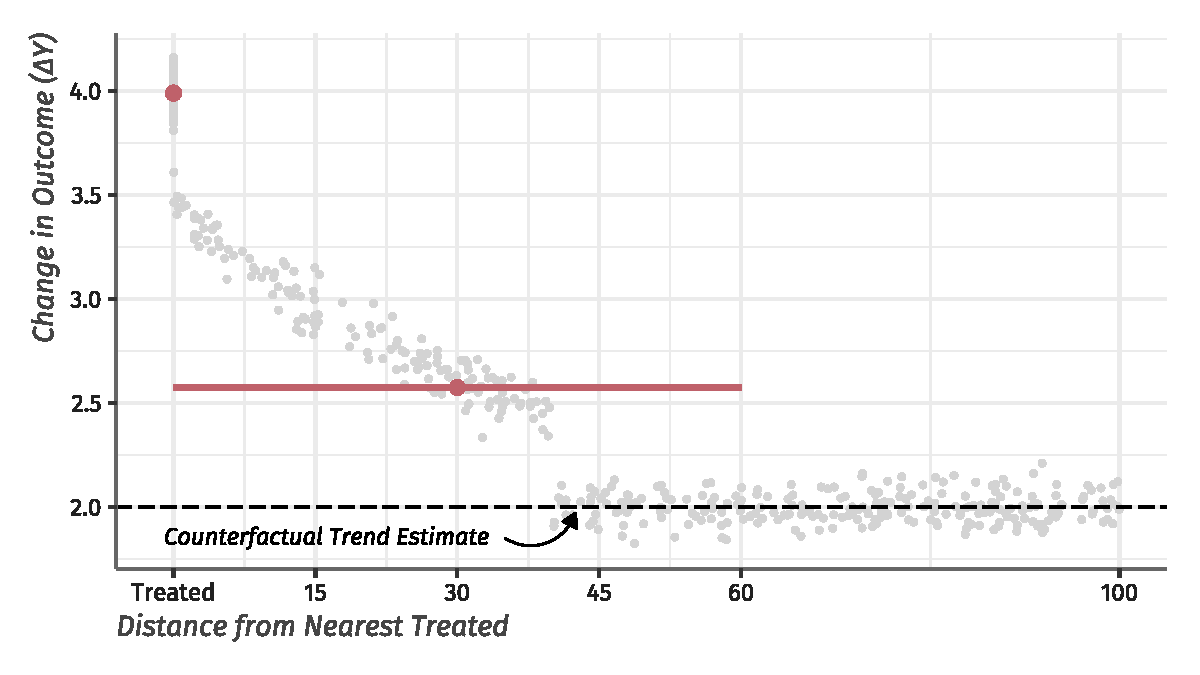
\includegraphics{../../figures/figure-within_example.pdf}
            }
        \end{center}
        
    \end{subfigure}
    \begin{subfigure}{\textwidth}
        \caption{Multiple Rings}
        \begin{center}
            \resizebox{0.8\textwidth}{!}{
                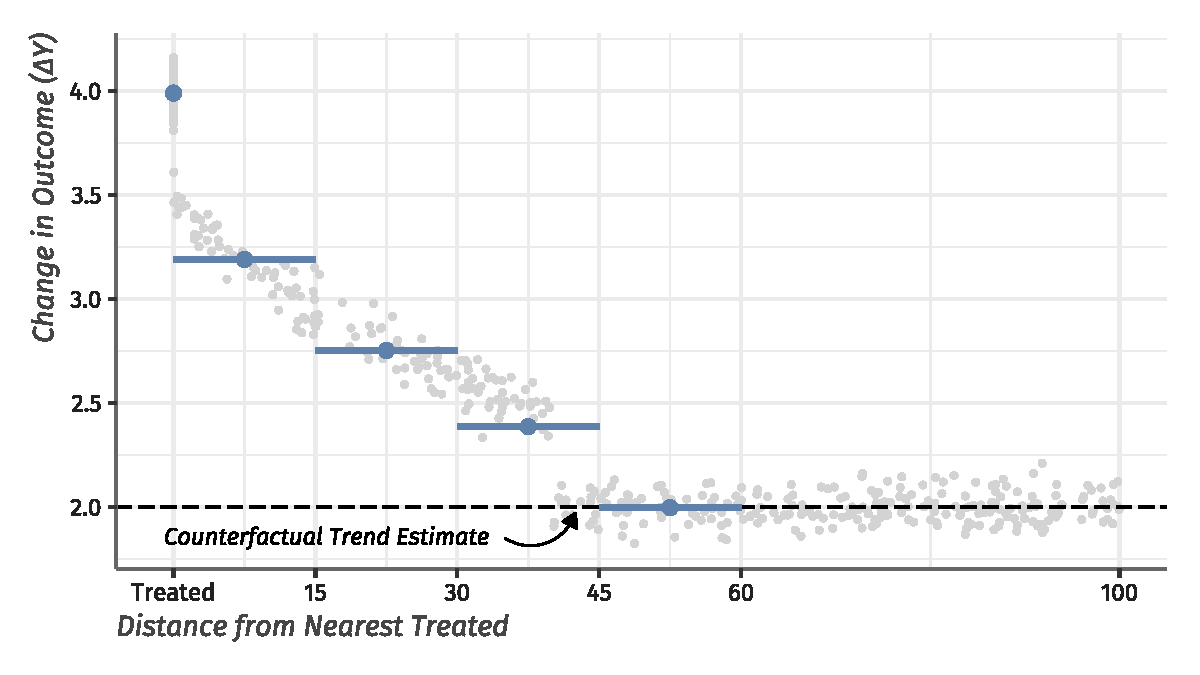
\includegraphics{../../figures/figure-rings_example.pdf}
            } 
        \end{center}
    \end{subfigure}

    \noindent{\footnotesize \textit{Notes:} Panel (a) shows the estimate of a single large ring indicator following equation (\ref{eq:twfe_with_ind}). Panel (b) shows a set of concentric ring indicators following equation (\ref{eq:twfe_with_ind}) where $S_{i}$ is replaced with a set of ring indicators.}
\end{figure}

An improvement on this is to use a set of concentric ring indicators instead of a single large ring indicator to more flexibly estimate the spillover effects (e.g 0-20 miles, 20-40 miles and 40-60 miles from the nearest treated unit). Since the set of rings is collinear with a single large ring, the direct effect estimate retains its unbiased properties, while spillover effects can potentially be estimated more accurately. A simple example of how rings improves estimation of spillover effects can be seen in Figure \ref{fig:example_rings}. The figure displays observations of $\bar{Y}_{i,Post} - \bar{Y}_{i,Pre}$ on the y-axis and the distance to the nearest treated unit on the x-axis and treated units are placed at a zero distance for visualization purposes. The example has a counterfactual trend of 2 so any difference from 2 is due to either treatment/spillover effects and the error term. Panel (a) uses a single indicator for being between 0 and 60 miles from treatment and the difference between the bar and the estimated counterfactual trend is the estimated spillover effect which in this case is about 0.6. This number masks that units within the first 15 miles have a treatment effect of 1 or larger and units between 40 and 60 miles have 0 spillover effects. 

Figure (b) on the other hand uses 4 indicators for every 15 mile interval (0-15, 15-30, 30-45, and 45-60 miles). This improves on the estimate of a single ring in two ways. Multiple rings are better able to capture the evolution of spillover effects over distance. Furthermore, the ring that is included past the true maximum distance where spillover effects occur has a point estimate near zero. The rings method acts a semi-parametric estimator in the sense that as the number of rings increase and their width shrinks, the estimates would trace out the spillover effect function (subject to their being units outside of the rings). However, precision of estimates would decrease as the number of rings increase and therefore there is a bias-variance trade-off in the number and width of rings. \citet{Clarke_2017} proposes a cross-validation technique for optimally choosing the number of rings and their techniques that uses the out-of-sample mean square prediction error as a way to estimate the bias-variance tradeoff. Interested readers can see the paper for technical and implementation details.

One disadvantage of using a set of indicator for \textit{the nearest} treated unit is that some spillover effects are additive in the number of nearby treated units. In this case, summarizing exposure by the distance to the closest treated unit fails to capture important information on the location of other treated units and the coefficients on the ring indicators might be interpreted incorrectly. One potential solution is to count the number of treated units within each ring instead of creating indicators for nearest treated unit. This additive version of rings however no longer removes all bias from the direct effect of treatment unless the exposure mapping is correctly specified. Therefore, if spillover effects are expected to be additive in nature, seperate estimation of the direct effect and spillover effects would be the preferred method. 

% ------------------------------------------------------------------------------
\subsection{Monte Carlo Simulations}
% ------------------------------------------------------------------------------

% ------------------------------------------------------------------------------
\subsubsection{Bias Under Misspecification of Spillovers}
% ------------------------------------------------------------------------------

To illustrate the above discussion, I turn to a set of Monte Carlo simulations. The first exercise is to consider a set of different data generating processes and see how well estimates of the direct effect perform when controlling for spillovers using potentially misspecified exposure mappings. In the general form, I generate data with unit and time fixed effects and an error term that is uncorrelated with $D_{i,t}$ for many different exposure mappings $h(\vec{D}, i)$. I generate data for unit $i$ is a US county at time $t \in \{1, \dots, 20\}$ using the following data-generating process:
\begin{equation}\label{eq:dgp_general}
    y_{i,t} = \mu_t + \mu_i + 2 D_{i,t} + \beta_{\text{spill, control}} (1-D_{i,t}) h(\vec{D}, i) + \varepsilon_{i,t},
\end{equation}
where $\mu_t \sim N(0.2t, 0.1^2)$ and $\mu_i \sim N(6, 2^2)$ respectively and the error term is IID and distributed as $\varepsilon_{i,t} \sim N(0, 2^2)$. 

For simplicity, I also remove spillovers onto treated units, but the results of which specifications perform best in the simulation are the same. In order to keep the magnitude of bias constant across specifications, I normalize the average spillover magnitude to be equal across specifications.\footnote{This results in a constant bias for TWFE estimates across data-generating processes.} For each true data-generating process, I estimate (\ref{eq:dgp_general}) with the correct spillover and misspecified alternatives $\tilde{h}(\vec{D}, i)$. 

The set of spillover specifications included in the data-generating process are `Within $40/80$mi.' which equals 1 if the counties' center of population is within $40/80$ miles to a treated county's center of population. `Within $40/80$mi. (Additive)' is the number of treated county's within $40/80$ miles of the control county. `Decay' is given by $\max_j D_j e^{-0.02 d(i,j)} * 1(d(i,j) < 80)$ and `Decay (Additive)' is given by $\sum_{j \neq i} D_j \exp^{-0.02 d(i,j)}$.

The last set of spillover specifications is commonly used in the literature as a semi-parametric estimator and are referred to as `Rings'. These consist of a set of indicators for falling within distance bins from the nearest treated unit (e.g. indicators for being between 0-20, 20-40, 40-60, and 60-80 miles to closest treated unit). The last specification is an additive version of `Rings' which is the number of treated units within each distance bin. This maintains a lot of the intuitive advantages of the `Rings' specification but parameterizes the spillovers to be additive in the number of nearby treated units. The advantage of this, as seen below, is enhanced performance of estimating spillover effects that are additive in nature. However, if the true specification is non-additive, then the additive specification no longer will remove all the bias from the direct effect estimate.

% Bias Table
\begin{table}[!tb]
    \caption{Bias from Misspecification of Spillovers}
    \label{tab:misspecification}
    \renewcommand\arraystretch{1}

    \begin{adjustbox}{width = 1.1\textwidth, center}
        \begin{threeparttable}
            \begin{tabular}{@{} l *{6}{d{2.4}} @{}}
                % Head
                \toprule
                & \multicolumn{6}{c}{Data-Generating Process} \\
                \cmidrule{2-7}

                & \mcl{\textbf{Within 40mi}} & \mcl{\textbf{Within 80mi}} & \mcl{\textbf{Within 40mi.}} & \mcl{\textbf{Within 80mi.}} & \mcl{\textbf{Decay}} & \mcl{\textbf{Decay}} \\
                Specification & & & \mcl{\textbf{(Additive)}} & \mcl{\textbf{(Additive)}} & & \mcl{\textbf{(Additive)}} \\
 
                % Body
                \midrule
                
                
TWFE (No Spillovers)                                   & 0.263   & 0.263   & 0.263   & 0.263   & 0.263   & 0.263   \\
                                                       & [0.091] & [0.091] & [0.091] & [0.091] & [0.091] & [0.091] \\
Within 40mi.                                           & 0.000   & 0.219   & 0.164   & 0.000   & 0.182   & 0.149   \\
                                                       & [0.022] & [0.070] & [0.049] & [0.022] & [0.055] & [0.044] \\
Within 80mi.                                           & 0.000   & 0.000   & 0.000   & 0.000   & 0.000   & 0.000   \\
                                                       & [0.024] & [0.024] & [0.024] & [0.024] & [0.024] & [0.024] \\
Within 40mi. (Additive)                                & 0.049   & 0.227   & 0.179   & -0.001  & 0.183   & 0.149   \\
                                                       & [0.025] & [0.074] & [0.054] & [0.022] & [0.055] & [0.044] \\
Within 80mi. (Additive)                                & 0.043   & 0.142   & 0.107   & -0.004  & -0.001  & -0.003  \\
                                                       & [0.025] & [0.043] & [0.034] & [0.023] & [0.023] & [0.023] \\
Decay                                                  & -0.151  & 0.079   & 0.000   & -0.166  & 0.024   & -0.024  \\
                                                       & [0.046] & [0.030] & [0.024] & [0.051] & [0.024] & [0.024] \\
Decay (Additive)                                       & -0.015  & 0.155   & 0.095   & -0.077  & 0.026   & -0.001  \\
                                                       & [0.023] & [0.047] & [0.032] & [0.029] & [0.024] & [0.023] \\
Rings (0-20, 20-30, 30-40)                             & 0.000   & 0.219   & 0.164   & 0.000   & 0.182   & 0.149   \\
                                                       & [0.022] & [0.070] & [0.049] & [0.022] & [0.055] & [0.044] \\
Rings (0-20, 20-30, 30-40, 40-60, 60-80)               & 0.000   & 0.000   & 0.000   & 0.000   & 0.000   & 0.000   \\
                                                       & [0.024] & [0.024] & [0.024] & [0.024] & [0.024] & [0.024] \\
Rings (0-20, 20-30, 30-40, 40-60, 60-80) (Additive)    & 0.044   & 0.142   & 0.108   & -0.001  & -0.001  & -0.001  \\
                                                       & [0.025] & [0.043] & [0.035] & [0.023] & [0.023] & [0.023] 
                
                \\ \bottomrule
            \end{tabular}
            
            % Notes 
            \begin{tablenotes}\footnotesize
                \item \textit{Notes.} Each cell corresponds to the results from 1000 simulations of the data generating process specified by the column header and estimated by equation (\ref{eq:dgp_general}) with $\tilde{h}(\vec{D},i)$ given by the row label. The non-bracketed number represents the mean bias from the simulations and the bracketed number represents the mean square error given by $\sum_{i = 1}^n \frac{(\hat{\tau}_i - \tau_0)^2}{n}$
            \end{tablenotes}
        \end{threeparttable}
    \end{adjustbox}
\end{table}


The results of the simulations are produced in Table \ref{tab:misspecification}. For each entry in the table, the column label corresponds to the true exposure mapping used in the data-generating process and the row label corresponds to the exposure mapping, $\tilde{h}(\vec{D}, i)$, used in estimation.  The corresponding cell gives the mean bias from estimating equation (\ref{eq:dgp_general}) with the $\tilde{h}(\vec{D}, i)$ given by the row. The bracketed number below the mean bias is the mean-squared error of the estimate which is given by $\sum_{i=1}^n \frac{(\hat{\tau}_{i,\text{direct}} - \tau_0)^2}{n}$. The mean squared error combines the square of the bias term, the variance of the estimator, and the variance of the error term which does not depend on the equation specification. This measure gives a good sense of the trade-off with whether decreasing bias comes at the cost of increasing the variance of the estimator.

The first thing to note is that all specifications remove a large portion of the bias relative to traditional two-way fixed effect estimate and lower the mean-squared error. In particular, correctly specifying the data-generating process removes almost all the bias in the direct effect estimate and greatly lowers the mean-squared error.  

The second result is that both the non-additive `Rings' and the `Within' specification perform best among all the misspecified spillovers in terms of removing bias, so long as they are wide enough to capture all the spillovers. This is due to the fact that indicator variables will correctly identify the average spillovers onto control units if they cover all the effected control units (see Proposition \ref{thm:remove_bias}). They also do so without increasing the variance of the estimator relative to the true specification, as shown by comparing the mean-squared errors. However, if the indicator is not wide enough as is the case with Within 40mi. for the 80mi. data-generating process, bias remains in the estimates. Therefore, if researchers are primarily interested in identifying the direct effect, then either `Rings' or `Within' specifications with a large cutoff distance are preferred as they remove almost all bias in all settings. 

% ------------------------------------------------------------------------------
\subsubsection{Spillover Effect Estimation}
% ------------------------------------------------------------------------------

Now, I turn to analyzing how the specifications perform at estimating the spillover effects themselves. For the next table, I predict the spillover effect for each control unit from the point estimates on $\tilde{h}(\vec{D}, i)$. Then as a measure for how well spillovers are estimated, I will calculate one minus the mean squared prediction error normalized by the sum of squared spillovers (for comparison across data-generating processes), \[ 
    1 - \frac{\sum_{i: D_i = 0} (\beta_{\text{spill, control}} h(\vec{D}, i) - \hat{\beta}_{\text{spill, control}} \tilde{h}(\vec{D}, i))^2}{\sum_{i: D_i = 0} (\beta_{\text{spill, control}} h(\vec{D}, i))^2}.
\] This will produce a percentage of spillovers that are explained by the specification, so numbers closer to $100\%$ represent better modelling of the spillovers. 

% MSPE Table
\begin{table}[!tb]
    \caption{Percent of Spillovers Predicted by Specification}
    \label{tab:misspecification_mspe}

    \begin{adjustbox}{width = 1.1\textwidth, center}
        \begin{threeparttable}
            \begin{tabular}{@{} l *{6}{d{2.2}} @{}}
                % Head
                \toprule
                & \multicolumn{6}{c}{Data-Generating Process} \\
                \cmidrule{2-7}

                & \mcl{\textbf{Within 40mi}} & \mcl{\textbf{Within 80mi}} & \mcl{\textbf{Within 40mi.}} & \mcl{\textbf{Within 80mi.}} & \mcl{\textbf{Decay}} & \mcl{\textbf{Decay}} \\
                Specification & & & \mcl{\textbf{(Additive)}} & \mcl{\textbf{(Additive)}} & & \mcl{\textbf{(Additive)}} \\
 
                % Body
                \midrule
                
                
                TWFE (No Spillovers) & $0.0\%$ & $0.0\%$ & $0.0\%$ & $0.0\%$ & $0.0\%$ & $0.0\%$ \\ 
Within 40mi. & $99.3\%$ & $25.0\%$ & $58.8\%$ & $85.4\%$ & $38.4\%$ & $55.6\%$ \\ 
Within 80mi. & $39.5\%$ & $96.4\%$ & $85.7\%$ & $33.9\%$ & $71.5\%$ & $67.6\%$ \\ 
Within 40mi. (Additive) & $85.1\%$ & $20.5\%$ & $51.4\%$ & $99.5\%$ & $40.5\%$ & $60.6\%$ \\ 
Within 80mi. (Additive) & $45.5\%$ & $61.0\%$ & $70.5\%$ & $47.2\%$ & $98.3\%$ & $93.5\%$ \\ 
Decay & $60.1\%$ & $81.8\%$ & $97.4\%$ & $52.7\%$ & $75.5\%$ & $81.9\%$ \\ 
Decay (Additive) & $60.4\%$ & $55.6\%$ & $78.0\%$ & $63.8\%$ & $93.2\%$ & $98.4\%$ \\ 
Rings (0-20, 20-30, 30-40) & $98.4\%$ & $22.8\%$ & $58.2\%$ & $85.7\%$ & $37.1\%$ & $55.8\%$ \\ 
Rings (0-20, 20-30, 30-40, 40-60, 60-80) & $96.7\%$ & $91.9\%$ & $92.1\%$ & $84.2\%$ & $72.7\%$ & $78.4\%$ \\ 
Rings (0-20, 20-30, 30-40, 40-60, 60-80) (Additive) & $83.3\%$ & $56.6\%$ & $72.7\%$ & $97.6\%$ & $94.9\%$ & $94.8\%$
                
                \\ \bottomrule
            \end{tabular}
            
            % Notes 
            \begin{tablenotes}\footnotesize
                \item \textit{Notes.} Each cell corresponds to the results from 1000 simulations of the data generating process specified by the column header and estimated by equation (\ref{eq:dgp_general}) with $\tilde{h}(\vec{D},i)$ given by the row label. The number corresponds to the mean square prediction error of the spillover effect for each control unit normalized by the total variance of spillover effects, given by 
                \[ 
                    1 - \frac{\sum_{i: D_i = 0} (\beta_{\text{spill, control}} h(\vec{D}, i) - \hat{\beta}_{\text{spill, control}} \tilde{h}(\vec{D}, i))^2}{\sum_{i: D_i = 0} (\beta_{\text{spill, control}} h(\vec{D}, i))^2}.
                \]
            \end{tablenotes}
        \end{threeparttable}
    \end{adjustbox}
\end{table}

Results of this exercise are presented in Table \ref{tab:misspecification_mspe}. For each specification, correctly specifying the spillovers produces the best estimates for spillovers as expected. Among misspecified exposure mapping, `Rings' that are large enough to caputre all the spillovers perform better than all other specifications in all non-additive data-generating processes. On the other hand, when the spillovers are additive, the predicted spillovers from the non-additive ring specifications do not as accurately measure these spillovers as they did before.\footnote{Although the non-additive Rings do estimate between 70\% and 80\% of the spillover effects while maintaining complete removal of bias.} Non-additvie specifciations perform somewhat poorly at estimating spillovers in the additive data-generating processes, `Within (Additive)' and `Decay (Additive)'. The `Rings (Additive)' specification sucessfully predicts spillovers in both additive data-generating processes. 

Therefore there are two practical pieces of guidance from these simulations. First, for their ability to remove all bias, `Rings' should be the default used by researchers for estimating the direct effect of treatment. Second, the most important aspect of correctly estimating spillovers is to consider whether they are additive in the number of treated units or not. Researchers should use a version of Rings either way.


% ------------------------------------------------------------------------------
\subsection{Guide for Applied Researchers}
\label{sec:parameterize}
% ------------------------------------------------------------------------------

The above discussion yields to practical recommendations based on three questions, the answers to which will ultimately depend on the economic context being studied. 

\begin{enumerate}
    \item Researchers should consider whether control units and/or treated units experience effects from the treatment status of other units. For example, in the context of library construction, treated units likely do not experience spillovers while close control units do. In the context of factory openings which affects nearby labor markets regardless of treatment status, both control and treated units likely experience spillovers. 
    
    \item Researchers must decide how far the spillovers extend and whether the effect decays over distance. This should again be guided by the economic context of the research question. For example, things such as driving distance or access via public transportation can be helpful in deciding which units are `close enough' to experience spillovers. 

    Importantly, Proposition \ref{thm:remove_bias} shows that the researcher does not need to specify the exact functional form of spillovers in order to have unbiased estimates of the treatment effect provided that spillovers are `local' as in Assumption \ref{assumption:local}. If only the direct effect of treatment is of interest, than a single ring indicator that contains units within the maximum distance will suffice. On the other hand, if spillover effects are of interest themselves, then a set of concentric rings is preferred for the reasons given above. 

    \item Last, it is important for estimation to determine if the spillovers are additive or non-additive in nature. If the number of nearby treated units matter, then the exposure mapping should sum over nearby treated units in some way. For example, in the context of library construction, the number of neighbors with libraries does not change the size of the spillover for it is access to \textit{any} library that matters. In the context of factory openings, though, agglomeration economies imply that the spillovers are additive in nature. As illustrated in the Monte Carlo simulations, in order to accurately estimate spillovers requires correctly using a additive or non-additive version of the concentric rings. 
\end{enumerate}

% ------------------------------------------------------------------------------
\subsection{Application in Place-Based Policy Analysis}
\label{sec:tva}
% ------------------------------------------------------------------------------

To illustrate the importance of accounting for spatial spillovers in the estimation of treatment effects, I revisit the analysis of the Tennessee Valley Authority (TVA) in \citet{Kline_Moretti_2014}. The TVA program was a large-scale federal investment started in 1934 that focused on construction of dams and transportation canals in an attempt to modernize the Tennessee Valley's economy. By the end of WWII, the TVA became the largest single power supplier in the country and significantly lowered the cost of wholesale energy for factories.\footnote{More details on the program are found in \citet{Kline_Moretti_2014}. The effects on wholseale electricity are discussed in \citet{Kitchens_2014}.} With over \$20 Billion (in 2000 dollars) spent which is hundreds of dollars transferred per person in the Authority, the impacts are very likely to extend past the authority's borders. \citet{Kline_Moretti_2014} analysze a range of outcome variables, but for succinctness I use only (the log of) agricultural and manufacturing employment. Since the TVA primarily improved manufacturing industries through large-scale electrification, the authors predict that employment will grow in manufacturing and shrink in agricultural as workers switch to higher-paying manufacturing jobs. 

The analysis in \citet{Kline_Moretti_2014} begins by comparing changes in county-level outcomes from 1940 to either 1960 (short-run effects) or 2000 (long-run effects) between treated counties in the Authority and control counties outside. The primary specification is
\begin{equation}\label{eq:tva}
    y_{c, t} - y_{c, 1940} = \alpha + \text{TVA}_c \tau + X_{c, 1940} \gamma + (\varepsilon_{c, t} - \varepsilon_{c, 1940}),
\end{equation}
where $c$ denotes county, $\text{TVA}_c$ is an indicator variable for being in the Authority, $\text{Post}_t$ is an indicator for being in the post-period, and $y$ is a set of outcome variables (in logs).\footnote{The two-periods difference-in-differences regression is equivalent to a first-difference regression. The authors use an Oaxaca-Blinder estimator on the first differences and the results of \citet{Kline_2011} show that this estimator is equivalent to a weighted difference-in-differences estimate. The weights are the propensity scores from a linear probability model where the outcome variable is being in the TVA. The weights can be seen in Figure III of their text, but generally counties close to the TVA are slightly upweighted relative to uniform weights. Their estimator does not differ much from the standard difference-in-differences results since the weights are not that different from uniform weights.} Pre-treatment control variables, $X_{c,1940}$, are interacted with $\text{Post}_t$ to allow for places to be on different long-term trends.\footnote{See footnote 8 in \citet{Kline_Moretti_2014} for a full listing of control variables.} To improve the likelihood of the paralell trends assumption, they run a logistic regression to predict being in the TVA based on their set of control variables $X_{c,1940}$ and keep only observations in the top 75\% of predicted probability. The counties used in the sample are presented in Figure \ref{fig:tva_sample}.

\citet{Kline_Moretti_2014} estimate (\ref{eq:tva}) to identify the `local effect' of the TVA -- what I am calling the `direct effect'. However, their point estimates compare, in part, changes in outcomes in TVA counties with changes in outcomes for neighboring counties that likely were impacted by the large-scale program. Their identification strategy depends \emph{explicitly} on a parallel counterfactual trends assumption after controlling for covariates and \emph{implicitly} on the SUTVA assumption. 

In the paper, the authors discuss the nature of spillovers that can occur. For agriculture employment, the authors claim that improved wages in the Authority will draw agriculture workers out of nearby counties. Hence they predict a negative spillover. For manufacturing, the sign is ambiguous. There could be positive spillovers if electrification brought cheap power and agglomeration economies to the neighboring areas.\footnote{\citet{Duranton_Puga_2003} give theoretical motivations for different sources of agglomeration.} However, manufacturing could decline if firms chose to locate in the Authority that would have, in the absence of the program, decided to locate in nearby counties.\footnote{\citet{Cuberes_Desmet_Rappaport_2021} refer to the positive spillover effects as `urban access' and the negative spillover effecte as `urban shadows' and find descriptive evidence of these effects changing importance over time.} My methodology will allow me to empirically test these predictions in the data and remove their bias from the treatment effect estimates. 

By comparing counties inside the Authroity to counties on the other side of the border, the authors likely underestimate the negative effect on agricultural employment while the bias in the manufacturing effect is theoretically ambiguous. The authors do recognize the problem of these comparisons and remove counties that share borders with the authority's, but due to the scale of the program, the spillovers are likely to extend further than this. As discussed in Section \ref{sec:remove_bias}, bias in their estimate will likely remain even after dropping contiguous counties. The estimation strategy I present keeps the observations near the TVA while controlling for spillover effects in a more rigorous manner.  

\begin{figure}[tb!]
    \caption{TVA Effective Sample and Spillover Variables}
    \label{fig:tva_sample}

    {\centering
        \resizebox{\textwidth}{!}{
            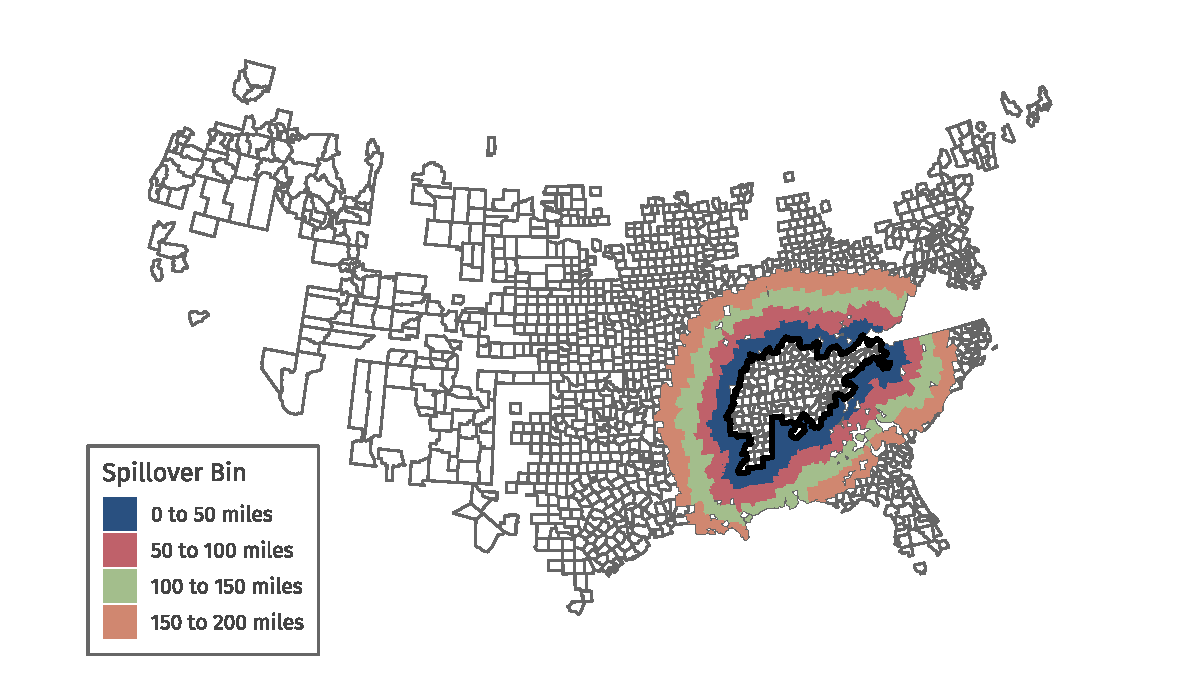
\includegraphics{../../figures/figure-tva-sample.pdf}
        } 
    }

    {\footnotesize \textit{Notes:} The above figure plots all the counties used in the estimation. Counties that fall within the distance intervals $\{ (0, 50], (50, 100], (100, 150], (150, 200] \}$ measured in miles are colored by their respective bin.} 
\end{figure}

I extend their analysis to control for spatial spillovers in the difference-in-differences specification. To parametrize the exposure mapping, I include a set of indicator variables for when a county is within a certain distance interval from the Authority. Specifically, I use the following intervals $\text{Dist} = \{(0, 50], (50, 100], (100, 150], (150, 200]\}$ measured in miles and define $\text{Between}(d)$ as an indicator for being within the interval $d \in \text{Dist}$ away from the Authority. Figure \ref{fig:tva_sample} displays the four spillover variables by filling in each distance bin in a different color. The magnitude and potentially the sign of spillovers can change with distance, hence I allow the effect to be seperately identified in bins. I keep the number of bins small to improve precision of spillover estimates. 

The specification with spillovers is given as follows:  
\begin{equation}\label{eq:tva_spillover}
    y_{i, t} - y_{i, 1940} = \alpha + \text{TVA}_i \tau + \sum_{d \in \text{Dist}} \text{Between}(d)\delta_d + X_{i, 1940} \beta + (\varepsilon_{i, t} - \varepsilon_{i, 1940}),
\end{equation} 
where $t \in \{1960, 2000\}$. The coefficients $\delta_d$ estimate the average spillover effect onto control units at different distances from the Authority. From proposition \ref{thm:remove_bias}, $\hat{\tau}$ will be an unbiased estimate for the `local' effect so long as spillovers do not occur past 200 miles from the TVA.

The results of the long-run analysis from 1940 to 2000 are presented in Panel A Table \ref{tab:tva}. The first column lists which dependent variable (measured in logs) was used in the row. The following columns contain point estimates for $\tau$ and $\delta_d$'s in different specifications. The point estimates can be interpreted as decadel growth rates in outcomes. The column labeled difference-in-differences uses an ordinary least squares estimator for the specification without spillovers, equation (\ref{eq:tva}). This estimate finds a decline in agricultural employment of about $5.1\%$ per decade and an increase in manufacturing employment of about $5.6\%$ per decade. 


% TVA Table
\begin{table}[!tb]
    \caption{Effects of Tennessee Valley Authority on Decadel Growth}
    \label{tab:tva}
    \renewcommand{\arraystretch}{1.1}

    \begin{adjustbox}{width = \textwidth, center}
        \begin{threeparttable}
            \begin{tabular}{@{} l c@{\extracolsep{20pt}}c@{\extracolsep{4pt}}cccc @{}}
                % Head
                \toprule

                & \multicolumn{1}{c}{\textbf{Diff-in-Diff}} & \multicolumn{5}{c}{\textbf{Diff-in-Diff with Spillovers}} \\ 
                \cmidrule{2-2} \cmidrule{3-7}
                & & & TVA between & TVA between & TVA between & TVA between \\ 
                & TVA & TVA & 0-50 mi. & 50-100 mi. & 100-150 mi. & 150-200 mi. \\ 
                \textit{Dependent Var.} & (1) & (2) & (3) & (4) & (5) & (6) \\
                
 
                % Body
                \toprule
                \multicolumn{7}{l}{\textbf{Panel A:} 1940-2000} \\
                \midrule
                
                 Population                  &    $0.0052$    &    $0.0053$    &    $-0.0040$   &    $-0.0212$   &    $-0.0077$   &    $-0.0053$   \\
                             &   $(0.0099)$   &   $(0.0090)$   &   $(0.0089)$   &   $(0.0179)$   &   $(0.0125)$   &   $(0.0123)$   \\
 Average manufacturing wage  &    $0.0064$    &  $0.0070^{**}$ &  $0.0075^{*}$  &    $0.0022$    &    $-0.0037$   &    $0.0023$    \\
                             &   $(0.0048)$   &   $(0.0030)$   &   $(0.0045)$   &   $(0.0047)$   &   $(0.0040)$   &   $(0.0047)$   \\
 Agricultural employment     & $-0.0561^{***}$& $-0.0514^{***}$& $-0.0678^{***}$& $-0.0310^{**}$ &    $-0.0112$   & $-0.0252^{***}$\\
                             &   $(0.0100)$   &   $(0.0087)$   &   $(0.0102)$   &   $(0.0123)$   &   $(0.0094)$   &   $(0.0084)$   \\
 Manufacturing employment    & $0.0606^{***}$ & $0.0560^{***}$ &  $0.0461^{**}$ &    $-0.0104$   &    $-0.0128$   &  $-0.0248^{*}$ \\
                             &   $(0.0170)$   &   $(0.0187)$   &   $(0.0210)$   &   $(0.0205)$   &   $(0.0257)$   &   $(0.0147)$   \\
 Value of farm production    &    $0.0024$    &    $-0.0060$   &    $-0.0184$   &    $-0.0188$   &    $-0.0101$   &    $-0.0266$   \\
                             &   $(0.0245)$   &   $(0.0269)$   &   $(0.0313)$   &   $(0.0252)$   &   $(0.0227)$   &   $(0.0176)$   \\
 Median family income        & $0.0219^{***}$ & $0.0191^{***}$ &  $0.0196^{**}$ &    $0.0056$    &    $-0.0062$   &    $-0.0011$   \\
                             &   $(0.0061)$   &   $(0.0067)$   &   $(0.0077)$   &   $(0.0079)$   &   $(0.0060)$   &   $(0.0032)$   \\
 Median housing value        &    $-0.0020$   &    $-0.0055$   &    $-0.0029$   &    $0.0039$    &    $0.0068$    &    $0.0006$    \\
                             &   $(0.0107)$   &   $(0.0091)$   &   $(0.0091)$   &   $(0.0163)$   &   $(0.0132)$   &   $(0.0063)$   \\


                \\ \toprule
                \multicolumn{7}{l}{\textbf{Panel B:} 1940-1960} \\
                \midrule 

                 Agricultural employment     & $0.0940^{***}$ &  $0.0856^{*}$  &    $-0.0062$   &    $-0.0042$   &    $-0.0303$   &    $-0.0039$   \\
                             &   $(0.0303)$   &   $(0.0498)$   &   $(0.0480)$   &   $(0.0480)$   &   $(0.0426)$   &   $(0.0359)$   \\
 Manufacturing employment    & $0.0894^{***}$ &  $0.0993^{**}$ &    $0.0228$    &    $0.0225$    &    $-0.0055$   &    $-0.0066$   \\
                             &   $(0.0324)$   &   $(0.0504)$   &   $(0.0496)$   &   $(0.0589)$   &   $(0.0384)$   &   $(0.0251)$   \\


                \\ \bottomrule
            \end{tabular}
            
            % Notes 
            \begin{tablenotes}\footnotesize
                \item \textit{Notes.} Each row corresponds to an outcome variable. Each cell is the point estimate and the standard error for the variable described in the column title. All standard errors are Conley standard errors with a correlation cutoff of 200 miles following \citet{Conley_1999}. The column labeled `Diff-in-Diff' estimates (\ref{eq:tva}) by OLS and is similar to the estimate reported in \citet{Kline_Moretti_2014}. The final four columns labeled `Diff-in-Diff with Spillovers' are estimates from (\ref{eq:tva_spillover}).
                
                \item $^{*} p< 0.1$; $^{**} p < 0.05$; $^{***} p < 0.01$.
            \end{tablenotes}
        \end{threeparttable}
    \end{adjustbox}
\end{table}

Turning to the specification that includes spillovers, equation (\ref{eq:tva_spillover}), column (2) contains a point estimate for $\tau$ and and columns (3)-(6) contain point estimates of the spillover effects $\delta_d$. For agricultural employment, the point estimates show there was a decline in agriculture employment in control units near the Authority. For control units between 0 and 50 miles, column (4) indicates a decline in agricultural employment of $3.7\%$ per decade. Between 50 and 100 miles the point estimate is $-1.6\%$ per decade, between 100 and 150 miles the point estimate is $-3\%$ per decade, and between 150 and 2000 miles the point estimate is $-1.6\%$ per decade. This is likely due to the fact that higher paying manufacturing jobs within the Authority drew farm-worker migrants from nearby counties. Because the spillovers onto the control counties is negative, the original difference-in-differences estimator was positively biased. The new point estimate indicates a decline of agricultural employment of about $7.4\%$ per decade compared to $5.1\%$ in the standard difference-in-difference specification. 

For manufacturing, our point estimates for spillovers are consistently negative, though imprecisely estimated in some columns. The spillover estimates suggest that neighboring counties experienced potentially negative spillover effects in the long-run. Since there are negative spillover effects present, the new point estimate in column (2) of $3.5\%$ is significantly smaller than the original estimate of $5.6\%$. The spillover estimates are evidence that in the long-run, urban shadow forces dominate the benefits of urban access. As you move away from the Tennessee Valley, the point estimates become more negative which suggest that the benefits of urban access vanish over distance faster than the costs of urban shadow.

To see how spillover effects from a large-scale place-based policy develop over time, Panel B in Table \ref{tab:tva} presents results for the effects of the Tennessee Valley in the short-run using outcome data in 1960. Unlike in the long-run, areas near the Tennessee Valley did not experience significant declines in agricultural employment in the short-run. Since our long-run analysis finds significant increases in high paying manufacturing employment in the Tennessee Valley, this result is consistent with long-run migration costs being lower than short-run costs.

For manufacturing, there are potentially positive increases in manufacturing employment within 100 miles of the Tennessee Valley authority and near zero effects between 100 and 200 miles. In the short-run, it appears that the effects of urban access and the cheap wholesale electricity dominated the effects of urban shadow. The effect of urban shadows can potentially be smaller in the short-run if operating firms are unlikely to relocate. Long-run effects can be larger as entrant firms change their location decision and operating firms are slowly replaced which is what the long-run spillover effect estimates suggest.

These results show that including spillovers in the estimation of direct treatment effects is potentially important and can lead to \emph{significant} differences in treatment effect estimates. Analysis of place-based policies that do not account for the fact that treatment effects can spillover beyond the borders of treated areas can potentially be biased. More, the spillover effects caused by place-based policies change over time as frictions can create delays in reoptimizing behavior. 

% ------------------------------------------------------------------------------
\subsection{Identification Strategies in Place-Based Analysis}
% ------------------------------------------------------------------------------

More generally, my framework provides important insights into identification strategies when analysizing the effects of place-based policies. There are two ways I contribute. First, \citet{Baum-Snow_Ferreira_2015} recognize the problem of spatial spillovers causing problems in identification and point to aggregation of units as a way to alleviate to the problem (e.g. aggregating census tracts to metropolitan areas). However, this approach collapses the three seperate effects which might each be of interest into a singular aggregate effect. I have shown that all three effects of place-based policies can be estimated under very general assumptions about the spillovers. Therefore, the methods propose simple ways to estimate treatment effects with non-aggregated data.

Second, my framework provides insight for different identification strategies often used in the literature. Since place-based policies are targeted to specific distressed areas, comparison units are often hard to find. Researchers have developed many identification strategies to find comparison units that are similar in terms of unobservables. First, researchers use border discontinuities to compare treated units to units just on the otehr side of the border. The rationale for this is that unobservables that could be correlated with treatment would evolve continuously across the border and so neighobring units would serve as valid comparisons. A different identification strategy compares approved and close but ultimately rejected applicants (e.g. \citet{}). Since both the treated and comparison groups likely are simliar due to the comparison group was close to being treated, unobservables should be balanced. A key difference in these identification strategies is the distance comparison units are from the treated area and therefore the former is more prone to bias due to spillovers than the latter.

For example, consider the analysis of the effects of federal Empowerment Zones. The federal Empowerment Zones are specially designated areas in high-unemployment areas. The program gives businesses located in the zone tax incentives and the goal of the program is to reduce unemployment and poverty. In the literature, there are a set of conflicting results with some papers suggesting that the Empowerment Zones do indeed reduce poverty rates and others finding near-zero effects.\footnote{See Table 1 of \citet{Neumark_Young_2019} for a summary of the various treatment effect estimates in the literature.} 

\citet{Busso_Gregory_Kline_2013} compare census tracts in Empowerment Zones to census tracts that qualified and were rejected from the program. The rejected tracts are not typically geographically near accepted Empowerment Zones which removes the concern of spatial spillovers affecting control units' change in outcomes. They find large significant reductions in poverty rates. Meanwhile, \citet{Neumark_Kolko_2010} compare census tracts in Empowerment Zones to census tracts within 1,000 feet of the Zone. These control counties are likely the ones that experience the largest spillover effects. They find near-zero effects on poverty. 

My framework can reconcile both of these results. If census tracts just outside the Empowerment Zones also benefit from the policy, then the estimates of \citet{Neumark_Kolko_2010} are attenuated towards zero. These two identification strategies of using rejected applicants or using bordering units as the control group are very common in the urban literature more generally \citep{Baum-Snow_Ferreira_2015}. My paper suggests that the former is the preferred strategy if spillovers occur onto nearby control units. Identification strategies that rely on geographically close control units as having similar unobservables should be used cautiously. If treatment effects spillover treatment border, then estimated treatment effects can be biased.



% ------------------------------------------------------------------------------
\section{Estimating Event Study with Spillovers}
\label{sec:event_study}
% ------------------------------------------------------------------------------

The intuition from how spillovers cause biases in estimates of the direct effect of treatment extend into the setting where there is staggered adoption in treatment. When treatment turns on for different units at different times, two-way fixed effect estimates can be viewed as a weighted sum of $2 \times 2$ difference-in-differences estimates.\footnote{Various forms for these weights are described in \citet{Goodman-Bacon_2018}, \citet{Sun_Abraham_2020}, and \citet{deChaisemartin_DHaultfoeuille_2019}. I do not recharacterize the weights in this article and guide interested readers to the source articles themselves.} Therefore the bias terms will be an identically weighted sum of the bias terms from the $2 \times 2$ estimates, assuming that the parallel counterfactual trends assumption (\ref{assumption:parallel}) holds. However, since weights on some of the $2 \times 2$ estimates can be negative, the sign of the spillover effects do not determine the sign of the weighted average of the spillover effects. This makes the bias from spillovers much more difficult to sign. 

In order to estimate treatment effects in the presence of spatial spillovers and staggered treatment timing, I will propose an estimation strategy that follows \citet{Callaway_SantAnna_2020} while incorporating spillovers directly into estimation. However, I do not cover all the technical assumptions and point the reader to the main text for these details. To begin, Callaway and Sant'Anna define a `cohort' $g$ as the set of units that recevie treatment starting in period $g$. Let $G_g$ be an idicator equal to one for all units where treatment starts at period $g$ and $C$ an indicator equal to one if the unit never receives treatment. Each cohort, $g$, will serve as the treated group for a set of $2\times 2$ difference-in-differences. For each period $t$ they define the `group-time average treatment effect', $ATT(g,t) = \expec{Y_t(g) - Y_t(0) \ \vert \ G_g = 1 }$, where $G_g$ is an indicator for starting treatment in year $g$. The potential outcome is indexed by $g$ to allow for treatment effects to differ depending on the initial treatment year.

Therefore in the context of spillovers, our equivalent term is the `group-time average direct effect' which will be defined as $$ 
    ATT_{\text{direct}}(g,t) = \expec{Y_t(g, 0) - Y_t(0, 0) \ \vert \ G_g = 1 },
$$ where the second term in potential outcomes represents an exposure mapping of $h(\vec{D}, i) = 0$. Similar to above, we modify the parallel trends assumptions given by Callaway and Sant'Anna to hold in the absence of exposure. 

\begin{assumption}[Parallel Counterfactual Trends on a ``Never-Treated'' Group]\label{assumption:parallel_es_never}
    $$
        \expec{Y_t(0, 0) - Y_{t-1}(0, 0) \ \vert \ G_g = 1 } = \expec{Y_t(0, 0) - Y_{t-1}(0, 0) \ \vert \ C = 1 } 
    $$ 
\end{assumption}

\begin{assumption}[Parallel Counterfactual Trends on ``Not-Yet-Treated'' Groups]\label{assumption:parallel_es_notyet}
    $$ 
        \expec{Y_t(0, 0) - Y_{t-1}(0, 0) \ \vert \ G_g = 1 } = \expec{Y_t(0, 0) - Y_{t-1}(0, 0) \ \vert \ D_s = 0, G_g = 0 }
    $$ 
\end{assumption}

The group-time average direct effect is the building block of analysis in the framework proposed by Callaway and Sant'Anna. Estimation of the group-time average direct treatment effect, $ATT_{\text{direct}}(g,t)$ depends on which parallel trends assumption a researcher use. The difference-in-difference estimate uses period $t$ outcomes as the post-period and some period $g - \delta$ as the pre-period where $\delta$ is the number of periods before initial treatment.\footnote{It is recommended that $g - \delta$ be the closest period before anticipation can occur. For example, if no anticipation is present in the setting, then $\delta = 1$ would be the recommended choice.} In the context of spillovers, the canoncial difference-in-differences estimation will have to be adjusted using a parameterized exposure mapping to prevent the bias detailed in the $2 \times 2$ setting. As shown in Section \ref{sec:estimation}, this can be done using a large `Within' indicator that is wide enough to capture all of the spillovers. If a researcher is using Assumption \ref{assumption:parallel_es_notyet}, then estimation will be done with a subsample containing treated units from group $g$ and all units that are in groups $g' > t$. If a researcher is using Assumption \ref{assumption:parallel_es_never}, then estimation will be done using a supsample containing only control units and units in group $g$.

Then, as detailed in C\&S, the $ATT(g,t)$ can be aggregated using different weights depending on the pararmeter of interest (see Table 1 of \citet{Callaway_SantAnna_2020}). These aggregations take the form of
\begin{equation*}
    \theta = \sum_{g} \sum_{t} w(g,t) ATT_{\text{direct}}(g,t)    
\end{equation*} 
Different weights produce different estimates for different average effects of interest, e.g. event study estimates, group-level average treatment effects (across time), or an aggergate treatment effect. Estimation and different aggregation of the direct effects can be done using the `did' package produced by C\&S where the the `Within' indicator is included as a covariate. It is important to note that exposure can change over time as new units are treated, so researchers should make sure to use the correct values for exposure mapping for each year $t$.  


% ------------------------------------------------------------------------------
\subsection{Estimation of Spillover Effects}
% ------------------------------------------------------------------------------

Estimation of the spillover effects is potentially much more difficult as estimation of continuous variables or multiple treatment variables in the presence of staggered treatment timing is still a work in progress and past the scope of this article. However, for a `Within' indicator, estimation can be done in much the same way as the direct effect but with more caution when constructing the samples for each $2 \times 2$ estimate. The `Within' indicator can be thought of as the treatment indicator and the sample would consist of only the never-treated units. The advantage of the `Within' indicator is that it will remove all bias from the direct effects estimates if the indicator extends far enough and will give an estimate of the average spillover effect. However, as mentioned above, a `Within' indicator does a poor job of estimating (a) the shape of spillover effects over distance and (b) spillover effects that are additive in the number of nearby treated units. Estimation of different exposure mappings is a task left for future research. 

Groups in this case will be defined by the period which `Within' first equals 1 for a given observation and estimation of $ATT(g,t)$ should use all observations where `Within' is equal to zero for period t and before. Then, estimation can be done assuming that all control units are on the same counterfactual trends in the absence of spillovers which is satisfied by Assumption \ref{assumption:parallel_es_never}. Therefore, estimation and aggregation can be done in much the same way as for the direct effect but on just the subsample of control units.


% ------------------------------------------------------------------------------
\subsection{Application on Community Health Centers}\label{sec:chc}
% ------------------------------------------------------------------------------

As an application of the above methods, I extend the analysis of \citet{Bailey_Goodman_Bacon_2015}. The authors study the creation of federal community health centers between 1965 and 1974 that provided \textit{primary} care to low-income communities. They test the hypothesis if access to low/no- cost health care services decreased mortality rates on the treated population. To answer this question, the authors use a common event-study framework to compare outcomes in treated counties to all other US counties by estimating the following specification 
\begin{equation}\label{eq:chc_es}
    Y_{jt} = \theta_j + X_{jt} \beta + \sum_{y = -7}^{-2} \pi_y D_j 1(t - T_j^* = y) + \sum_{y = 0}^{15} \tau_{y} D_j 1(t - T_j^* = y) + \varepsilon_{jt},
\end{equation}
where $T_j^*$ is the year the county establishes a community health center, $D_j$ is an indicator for being treated, $\theta_j$ is county fixed effects, and $X_{jt}$ contains a set of controls.\footnote{Controls include 1960 county characteristic trends, state-year fixed effects, and urban-group fixed effects. A full list can be found on page 1080 of \citet{Bailey_Goodman_Bacon_2015}.} The coefficents $\pi_y$ can be interpreted as tests of parallel pre-trends and $\tau_y$ can be interepreted as the treatment effect of a community health center $y$ years after establishment. 

\begin{figure}[tb!]
    \caption{Effects of Establishment of Community Health Centers}
    \label{fig:chc_es}
        
        {\centering
            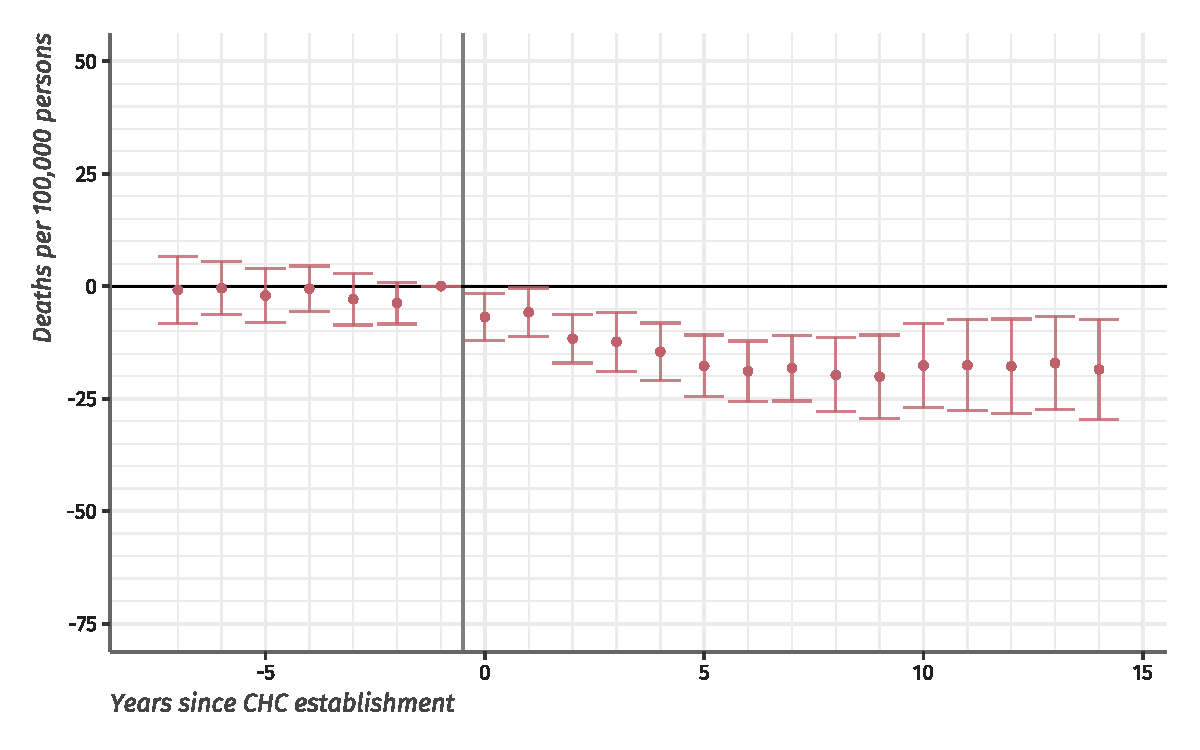
\includegraphics[width=\textwidth]{../../figures/figure-chc-es_original.pdf}
        }

    {\footnotesize
        \textit{Notes:} This figure recreates figure 5 from \citet{Bailey_Goodman_Bacon_2015}. Details on the event study specificaiton and controls can be found in the text.
    }
\end{figure}

The result are in Figure \ref{fig:chc_es}. Estimates of $\hat{\tau}_y$ show that counties that received health centers had significantly lower mortality rates than the other counties in the US. In years following the establishment of the community health centers, the authors find a reduction of between 15-30 deaths per 100,000 residents compared to a baseline adjusted mortality rate of 929 deaths per 100,000 residents. 

\begin{figure}[tb!]
    \caption{Direct and Spillover Effects of Community Health Centers}
    \label{fig:chc_es_spill}
        
        {\centering
            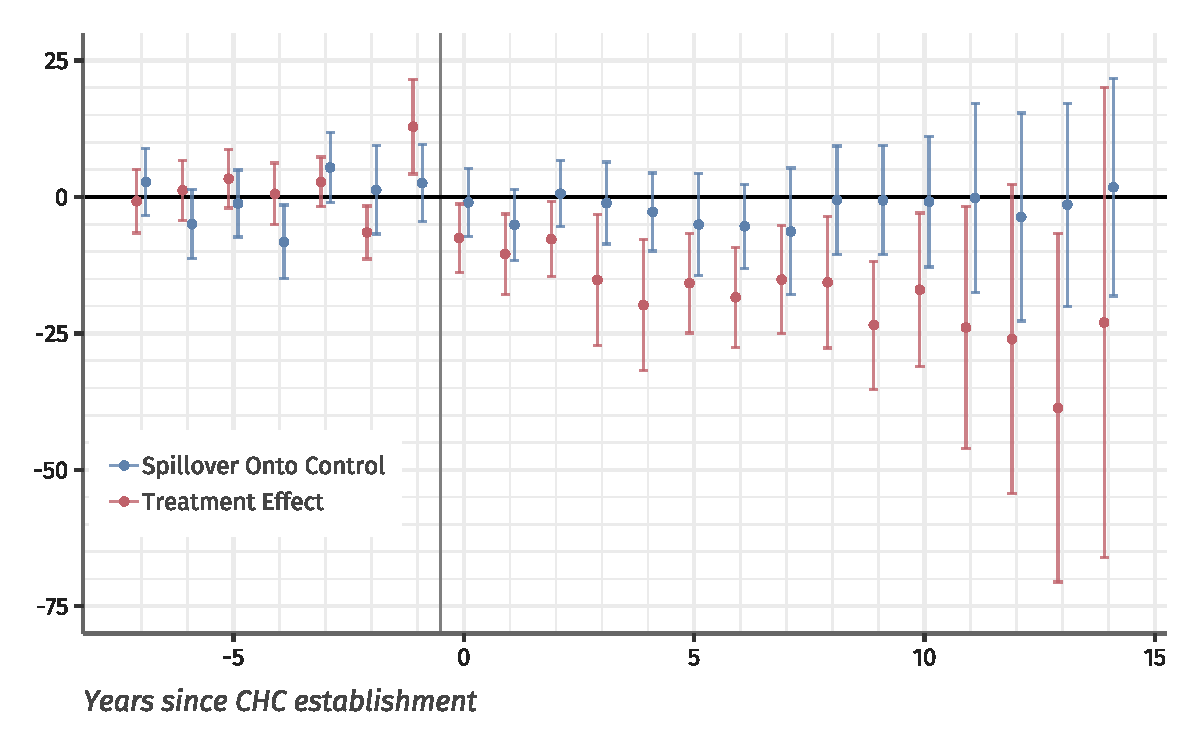
\includegraphics[width=\textwidth]{../../figures/figure-chc-es_combined.pdf}
        }

    {\footnotesize
        \textit{Notes:} This figure plots event study estimates for the treatment effect and the spillover effect on control units within 25 miles of treatment at different periods relative to establishment year. The estimates are generated using the `did' package produced from the paper \citet{Callaway_SantAnna_2020}. 
    }
\end{figure}

There are theoretical reasons to think spillovers may or may not exist in this context. On the one hand, individuals outside the county can potentially travel to the community health centers to receive care. This would create a negative spillover effect on mortality rates in nearby counties which would bias their estimates towards zero. On the other hand, \citet{Bailey_Goodman_Bacon_2015} document evidence that their estimated effects are not due to emergency but rather primary care services. In this case, it is less likely low-income individuals would travel very far to receive primary care and hence the spillover effects is potentially near zero. My methodology can provide an answer to the question of how far do individuals travel for low/no -cost primary care.

As in the method detailed above, I use the subsample of counties that do not receive a community health center and use an indicator for being within 25 miles of a treated county as the treatment variable. Then, I follow \citet{Callaway_SantAnna_2020} in estimating event-study coefficients. The results are presented in Figure \ref{fig:chc_es_spill}. The confidence intervals labeled with circles represent point estimates for the average spillover effect on control units within 25 miles. No spillover effect is estimated to be significantly different from zero which suggests that the effects of community health centers are very local. Since there are near zero spillover effects, the direct effect estimates marked in Figure \ref{fig:chc_es_spill} as diamonds maintain the same shape as the author's original estimates with estimates between 15-30 fewer deaths per 100,000 persons. 

The spillover effects results provide evidence that low-income individuals will not travel far to receive primary care. Practically, this suggests that community health centers should be targeted to be as accessible as possible for poor individuals as they are unable to travel far to access the services. 







% ------------------------------------------------------------------------------
\section{Conclusion}
\label{sec:conclusion}
% ------------------------------------------------------------------------------

This paper has considered the common environment where treatment is assigned via administrative boundary while the effects of treatment spread across these borders. In this context, difference-in-differences estimation will identify a combination of the direct effect of treatment and two additional terms resulting from spillovers. I have proposed a potential outcomes framework that formalizes spillovers. 

I use this framework to point to limitations in commonly used ad-hoc approaches to controlling for spillovers. Then, I propose a new estimation strategy that is robust to more forms of spillovers. In particular, I find that specifications with an indicator for being ``close to'' treated units interacted with treatment status will remove all bias in the direct effect estimate so long as all units affected by spillovers are contained in the indicator. More, I show that a set of concentric `rings' are the best at capturing the spatial structure of spillovers. When estimating spillover effects themselves, I find that it is important to correctly identify is spillovers are additive or non-additive in the number of nearby treated units.  

Then, I show that these approaches can change estimates significantly in the context of estimating the effects of place-based policies. Since place-based policies change the nature of agglomeration in the local and surrounding area --that is cause spillovers--local effects of these policies can be misestimated without controlling for spillovers. I also show the importance of considering spillovers in weighing the pros and cons of various identificatin strategies. Identification strategies based on geographic continuity of unobservables can magnify the bias from spillovers as they restrict the compairson group to observations experiencing the largest spillover effects.

Finally, I show how researchers can include spillovers in settings with variation in treatment timing following \citet{Callaway_SantAnna_2020}. I then use this method to show how considering spillovers in event-study framework provide additional insights for a researcher.








% ------------------------------------------------------------------------------
\newpage \bibliography{references.bib}
% ------------------------------------------------------------------------------


% ------------------------------------------------------------------------------
\newpage \appendix 
\renewcommand{\thetable}{\Alph{section}.\arabic{table}}
\renewcommand{\thefigure}{\Alph{section}.\arabic{figure}}
% ------------------------------------------------------------------------------

% ------------------------------------------------------------------------------
\section{Proofs}
\label{sec:proofs}
% ------------------------------------------------------------------------------

\textbf{Proof of Theorem \ref{thm:bias}}
\begin{align*}
    \expec{\hat{\tau} } &= \underbrace{\expec{\bar{Y}_{i,Post} - \bar{Y}_{i,Pre} \mid D_i = 1 } - \expec{\bar{Y}_{i,Post} - \bar{Y}_{i,Pre} \mid D_i = 0 }}_{\text{Difference-in-Differences}} \\
    &= \expec{\bar{Y}_{i,Post}(1, h(\vec{D}, i)) - \bar{Y}_{i,Pre}(0, \vec{0})  \mid D_i = 1 } - \expec{\bar{Y}_{i,Post}(0, h(\vec{D}, i)) - \bar{Y}_{i,Pre}(0, \vec{0}) \mid D_i = 0 } \\
    &= \expec{\bar{Y}_{i,Post}(1, h(\vec{D}, i)) - \bar{Y}_{i,Pre}(0, \vec{0})  \mid D_i = 1 } \\
    &\quad\quad - \expec{\bar{Y}_{i,Post}(0, h(\vec{D}, i)) + \bar{Y}_{i,Post}(0, \vec{0}) - \bar{Y}_{i,Post}(0, \vec{0}) - \bar{Y}_{i,Pre}(0, \vec{0}) \mid D_i = 0 } \\
    &= \expec{\bar{Y}_{i,Post}(1, h(\vec{D}, i)) - \bar{Y}_{i,Pre}(0, \vec{0})  \mid D_i = 1 } - \expec{\bar{Y}_{i,Post}(0, \vec{0}) - \bar{Y}_{i,Pre}(0, \vec{0}) \mid D_i = 0} \\ 
    &\quad\quad - \expec{\bar{Y}_{i,Post}(0, h(\vec{D}, i)) - \bar{Y}_{i,Post}(0, \vec{0})\mid D_i = 0} \\ 
    &= \expec{\bar{Y}_{i,Post}(1, h(\vec{D}, i)) - \bar{Y}_{i,Pre}(0, \vec{0})  \mid D_i = 1 } \\
    &\quad\quad - \expec{\bar{Y}_{i,Post}(0, \vec{0}) - \bar{Y}_{i,Pre}(0, \vec{0}) \mid D_i = 1} \\
    &\quad\quad - \expec{\bar{Y}_{i,Post}(0, h(\vec{D}, i)) - \bar{Y}_{i,Post}(0, \vec{0})\mid D_i = 0} \\  
    &= \expec{\bar{Y}_{i,Post}(1, h(\vec{D}, i)) - \bar{Y}_{i,Pre}(0, \vec{0}) - \bar{Y}_{i,Post}(0, \vec{0}) + \bar{Y}_{i,Pre}(0, \vec{0})\mid D_i = 1 } \\
    &\quad\quad - \expec{\bar{Y}_{i,Post}(0, h(\vec{D}, i)) - \bar{Y}_{i,Post}(0, \vec{0})\mid D_i = 0}\\
    &= \expec{\bar{Y}_{i,Post}(1, h(\vec{D}, i)) - \bar{Y}_{i,Post}(0, \vec{0}) \mid D_i = 1 } - \expec{\bar{Y}_{i,Post}(0, h(\vec{D}, i)) - \bar{Y}_{i,Post}(0, \vec{0})\mid D_i = 0}\\
    &= \expec{\bar{Y}_{i,Post}(1, h(\vec{D}, i)) + \bar{Y}_{i,Post}(1, \vec{0}) - \bar{Y}_{i,Post}(1, \vec{0}) - \bar{Y}_{i,Post}(0, \vec{0})\mid D_i = 1 } \\
    &\quad\quad - \expec{\bar{Y}_{i,Post}(0, h(\vec{D}, i)) - \bar{Y}_{i,Post}(0, \vec{0})\mid D_i = 0} \\
    &= \expec{\bar{Y}_{i,Post}(1, \vec{0}) - \bar{Y}_{i,Post}(0, \vec{0}) \mid D_i = 1} + \expec{\bar{Y}_{i,Post}(1, h(\vec{D}, i)) - \bar{Y}_{i,Post}(1, \vec{0}) \mid D_i = 1} \\
    &\quad\quad - \expec{\bar{Y}_{i,Post}(0, h(\vec{D}, i)) - \bar{Y}_{i,Post}(0, \vec{0}) \mid D_i = 0} \\
    &= \tau_{\text{direct}} + \tau_{\text{spill,treated}} - \tau_{\text{spill,control}} \\
\end{align*}



% ------------------------------------------------------------------------------
\section{Details on Dropping Control Unit Approach}
\label{sec:monte_carlo}
\setcounter{figure}{0}
\setcounter{table}{0}
% ------------------------------------------------------------------------------

I use the set of counties in the contiguous United States and the data generating process used is defined by the exposure mapping given in (\ref{eq:h_within}) with cutoff distance $\bar{d} = 40$ miles and the data generating process given in (\ref{eq:example_po}). A unit of observation is a US county and the periods are $t \in \{1, \dots, 20\}$ with treatment turning on after period $t = 10$. The unit and time fixed effects are generated by $\mu_t \sim N(0.2t, 0.1^2)$ and $\mu_i \sim N(6, 2^2)$ respectively, and the error term is $\varepsilon \sim N(0, 2^2)$. Last, the size of treatment and spillovers are as follows: $\beta_{\text{direct}} = 2$, $\beta_{\text{spill, control}} = 1$ and $\beta_{\text{spill, treat}} = 0$.

This data generating process where spillovers only occur onto control units matches what has been typically assumed in the literature. I assign treatment among counties randomly with various unconditional probabilities between 3 percent and 50 percent. The data-generating process is therefore 
\begin{equation}
    \label{eq:dgp1} 
    y_{i,t} = \mu_t + \mu_i + \beta_{\text{direct}} D_{i,t} + \beta_{\text{spill, control}} (1-D_{i,t}) \text{Near}_{i,t} + \varepsilon_{i,t}   
\end{equation}


\begin{figure}[tb!]
    \caption{Effectiveness of Removing `Contaminated' Control Units}
    \label{fig:bias_drop_control}
    

    \begin{subfigure}[t]{\textwidth}
        \caption{Spillovers Effects \emph{only} on Control} \label{fig:bias_as_treat_prob}
        
        {\centering
            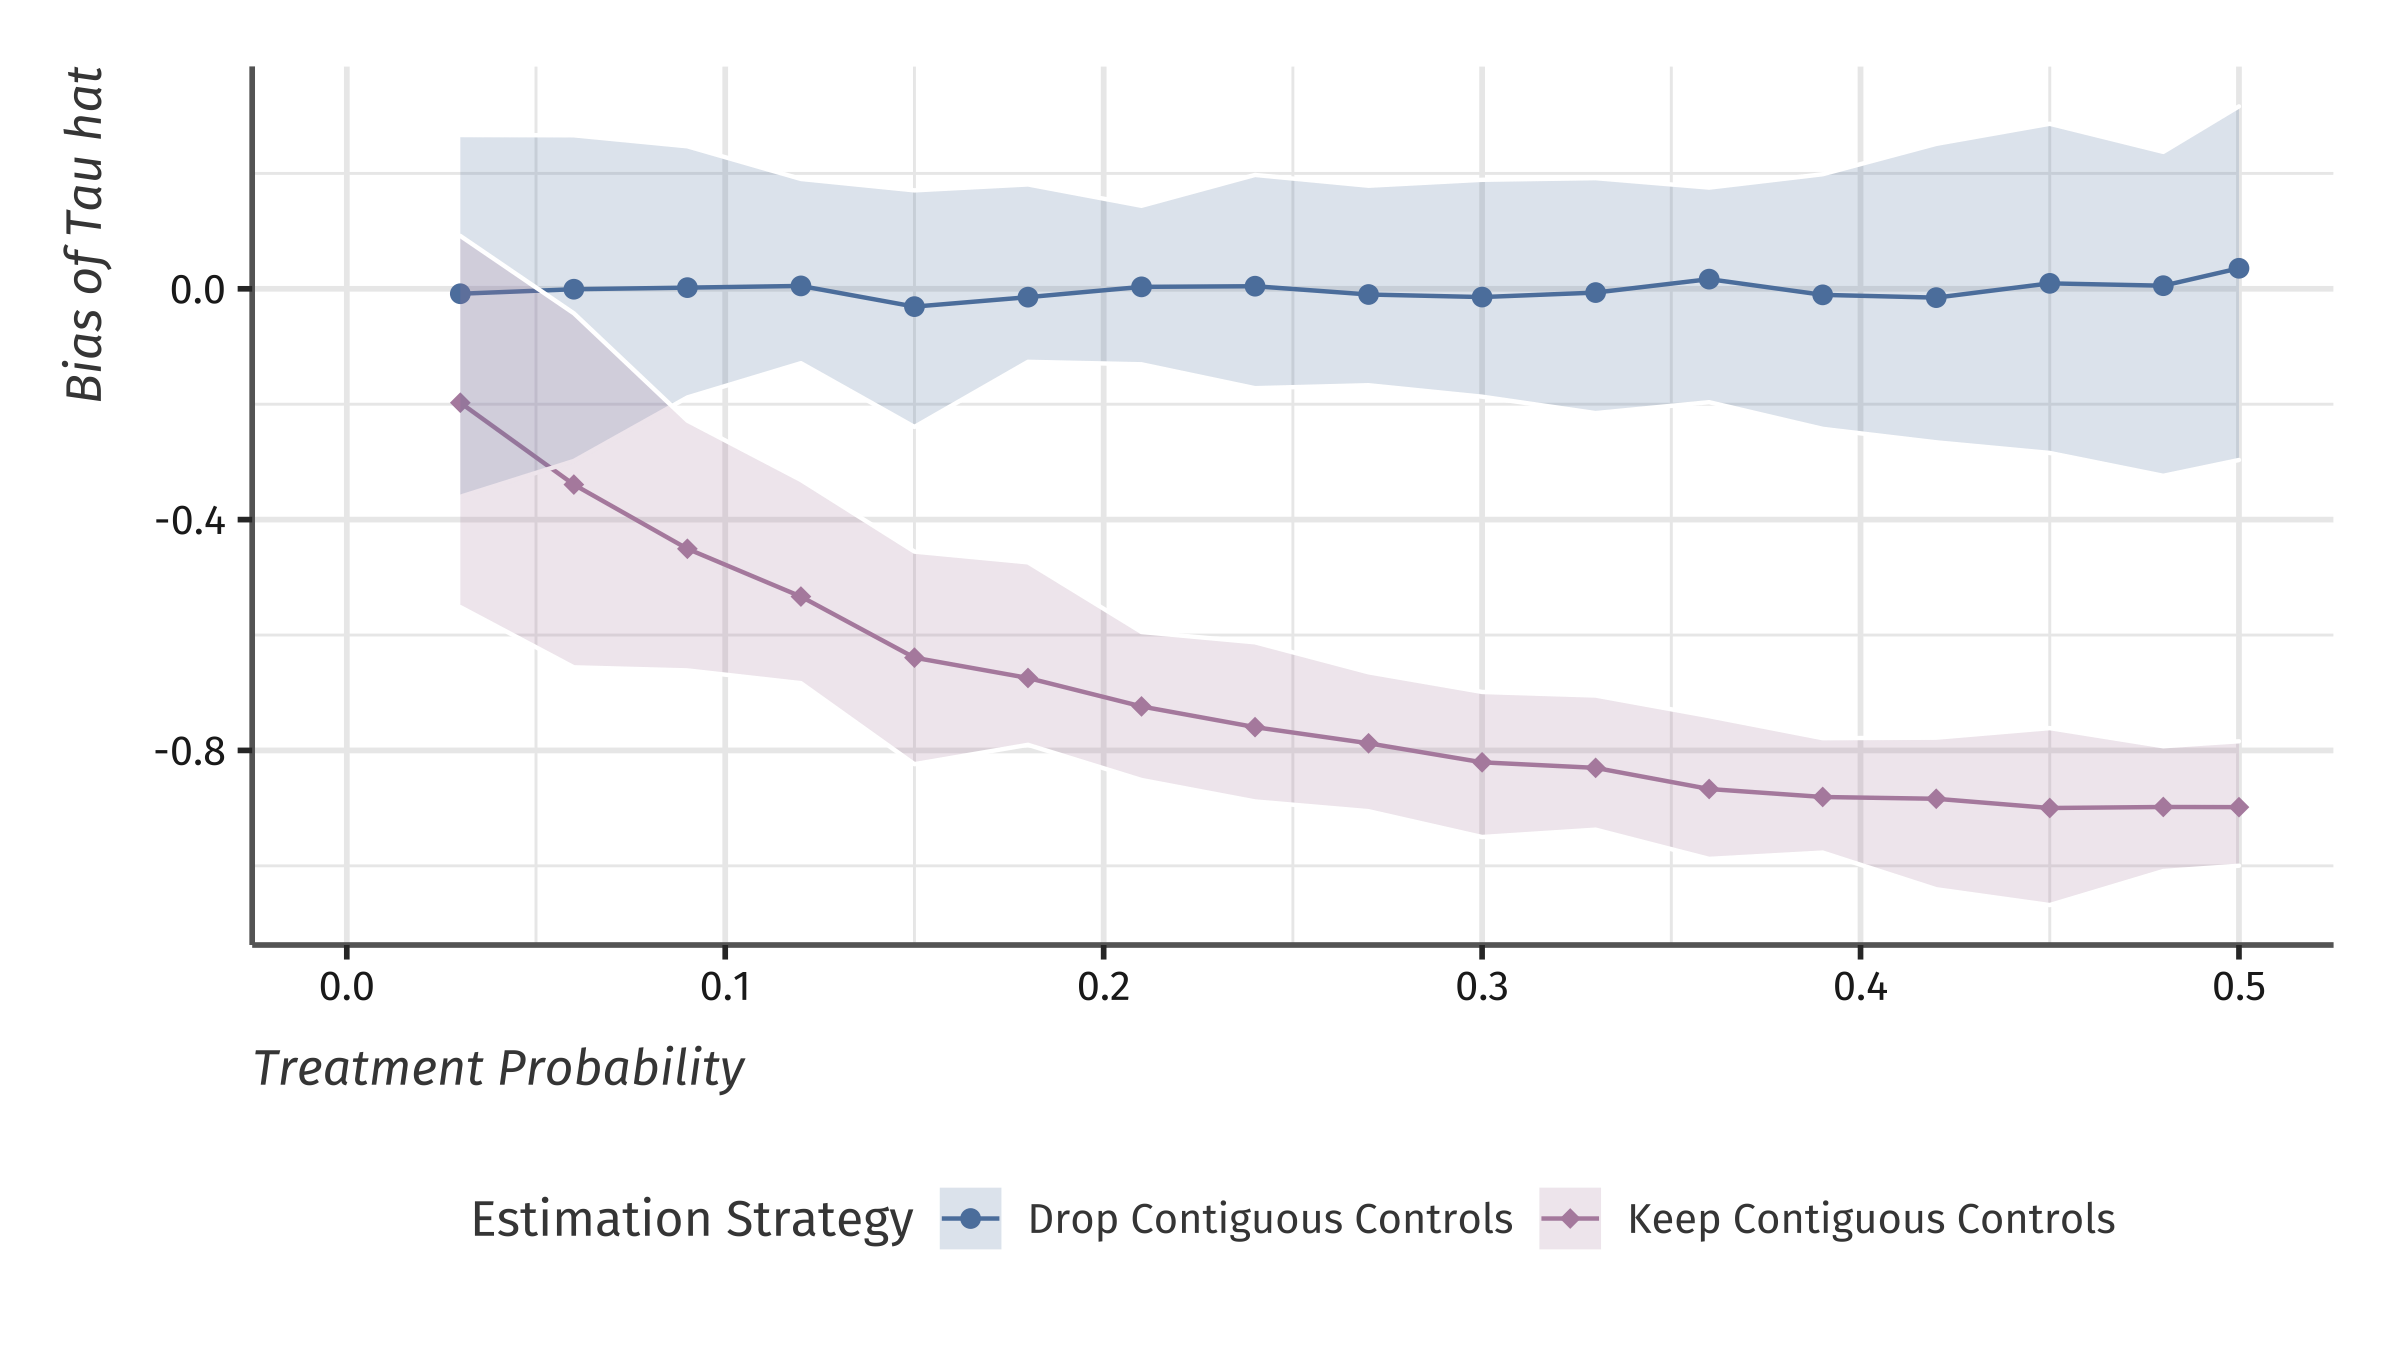
\includegraphics[width=0.9\textwidth]{../../figures/figure-bias_fix.png}
        }
    \end{subfigure}

    \begin{subfigure}[t]{\textwidth}
        \caption{Spillovers Effects on Control and Treated} \label{fig:bias_as_treat_prob_w_treat}
        
        {\centering
            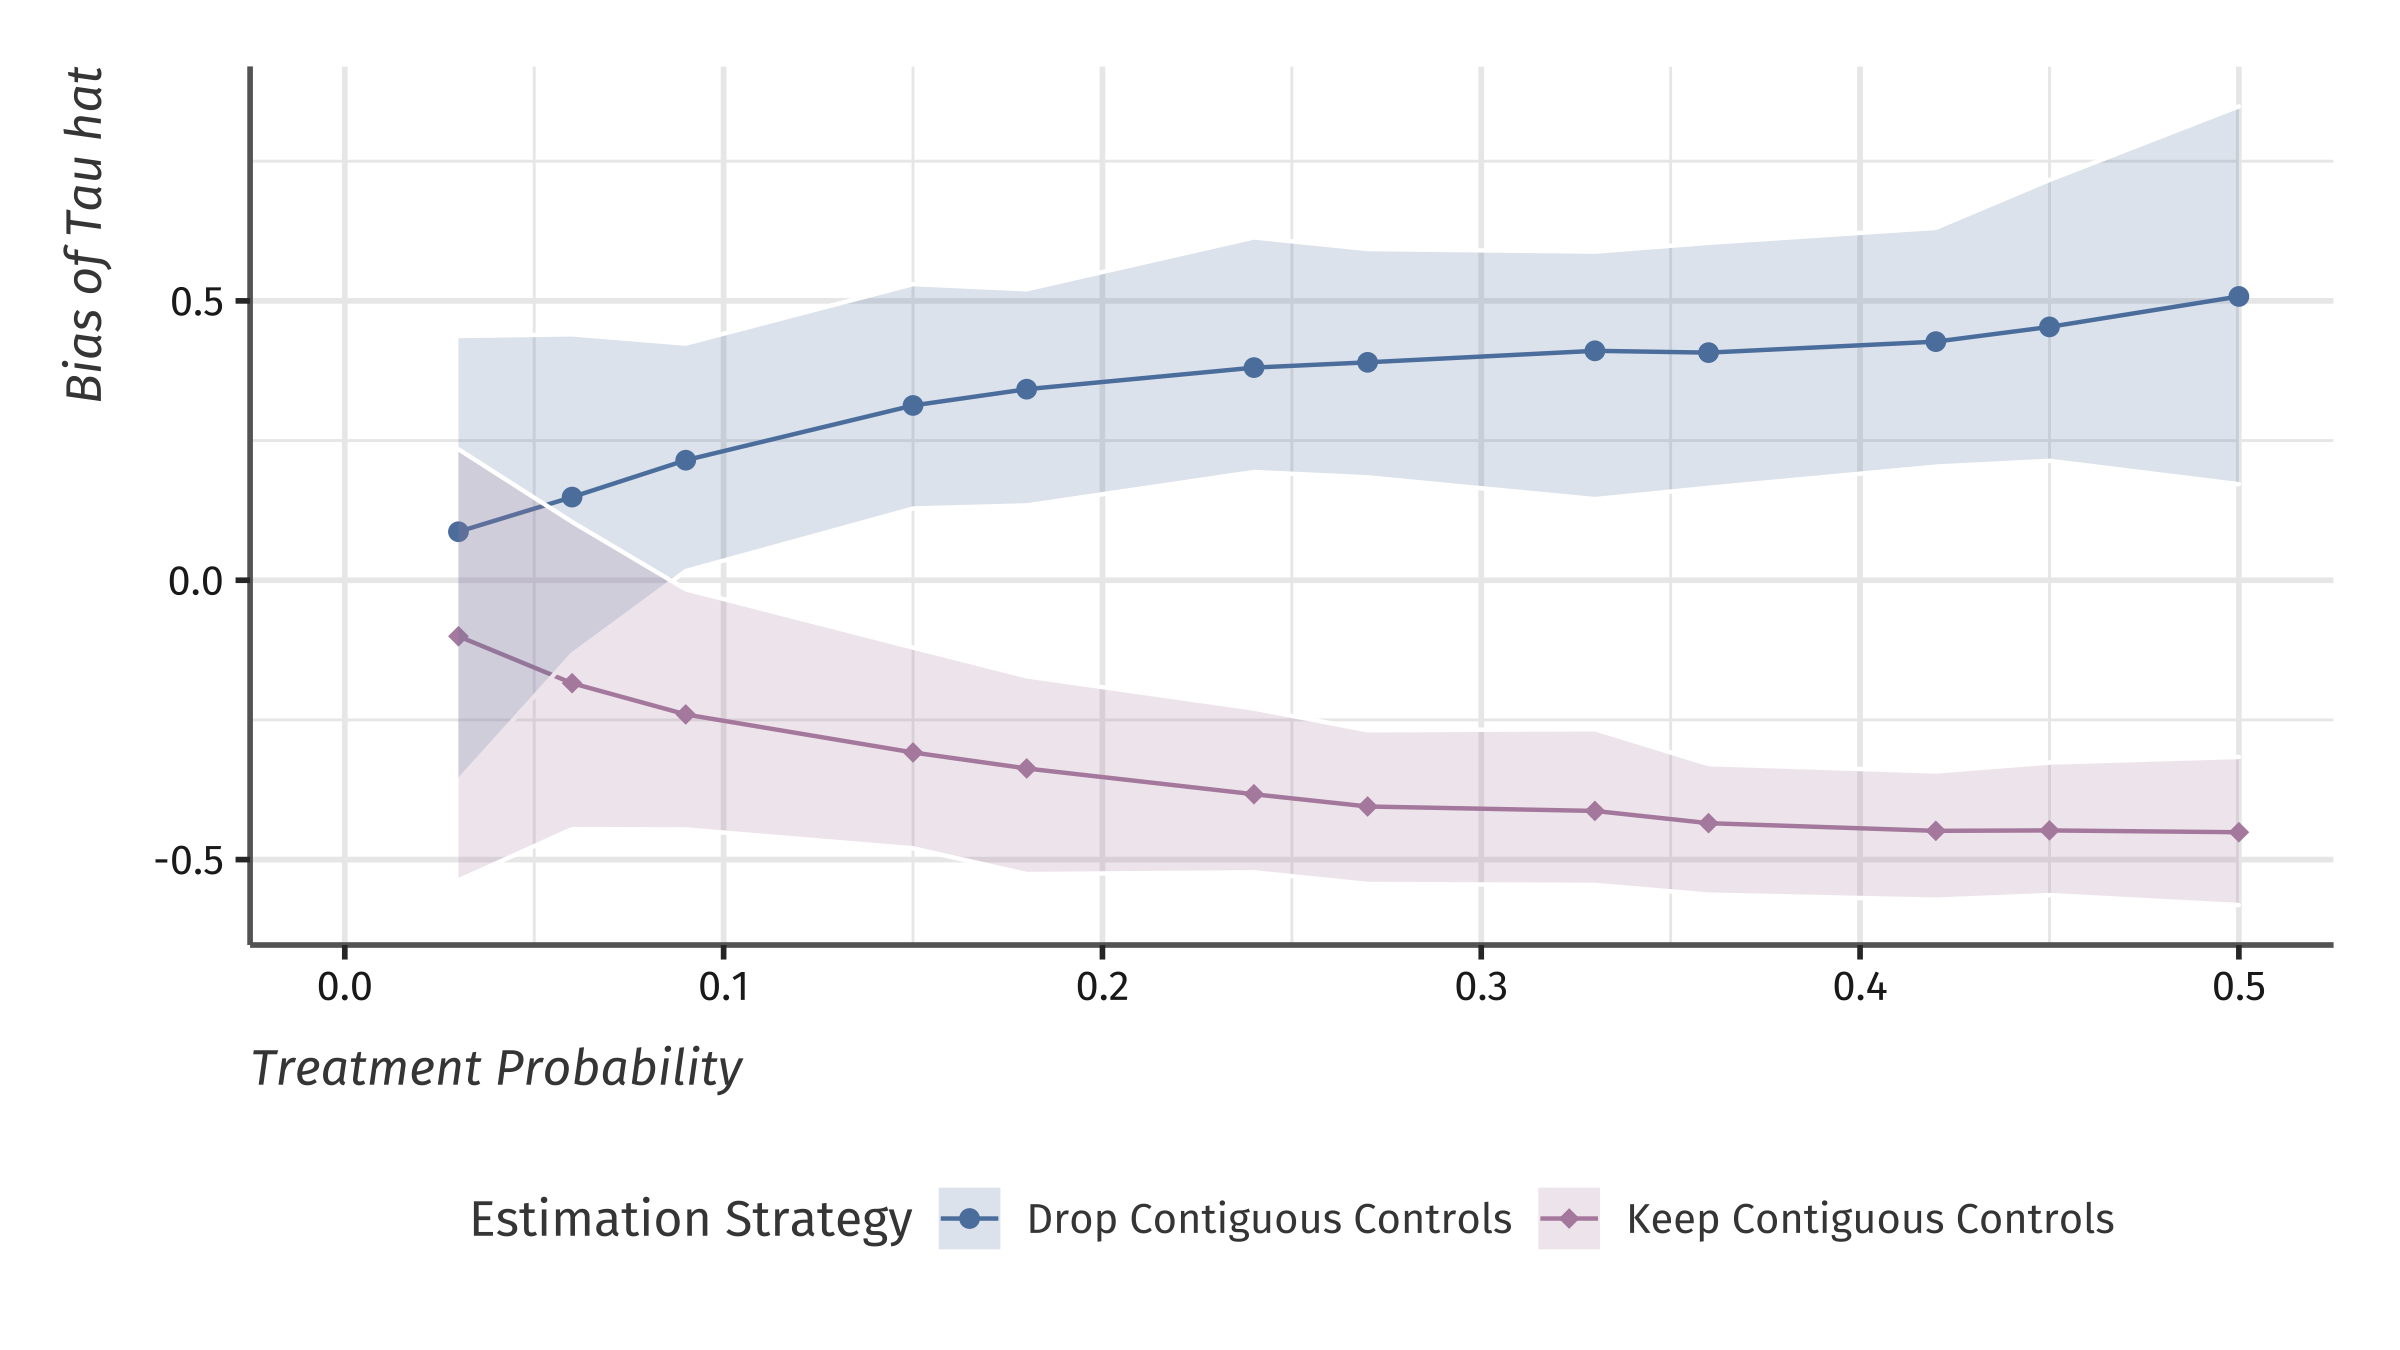
\includegraphics[width=0.9\textwidth]{../../figures/figure-bias_fix_treat.png}
        }
    \end{subfigure}

    {\footnotesize
        \textit{Notes:} This figure plots the bias of $\hat{\tau}$ found from estimating (\ref{eq:twfe}) for data generated as described in the text by equations (\ref{eq:dgp1}) for Panel A and (\ref{eq:dgp2}) for Panel B. Each point corresponds to the average bias for the given treatment probability and the band is the 95 percent empirical confidence interval over 1000 simulations. The line with diamond markers estimates with all control units. The line with circle markers removes control units that share a border with a treated county. 
    }
\end{figure}

The size of the bias from estimating the two-fixed effects model, (\ref{eq:twfe}), at different treatment probabilities are presented in Figure \ref{fig:bias_as_treat_prob} as the line with diamond markers. Each point represents a set of 10,000 simulation and displays the mean bias as well as a 95 percent empirical confidence interval. As displayed in the figure, even for a low treatment probability of three percent, the bias is quite large with a 95 percent empirical confidence interval between -0.28 and -0.75. As treatment frequency increases, the bias increases as well but at a slower rate due to fewer additional control units receiving spillover units. The slow increase in bias is in part due to the assumption that spillovers are not additive in the number of nearby units treated.

A common solution in the literature is to remove control units from the estimated sample that are most likely to be affected by spillovers. To do this, I remove contiguous control counties which is a close, but misspecificied, measure of $h(\vec{D}, i)$. The results are shown in Figure \ref{fig:bias_as_treat_prob} by the line with circle markers. Even though the exposure mapping is misspecified, contiguous counties approximates the true exposure mapping well enough such that the bias stays centered constantly around zero as most control units experiencing spillovers are removed. However, if the distance cutoff $\bar{d}$ were larger, more control units would remain in the sample that experience non-zero exposures. In this case, the bias would fall between the two lines.

There is a trade-off between the bias and the variance of the estimator when using this methodolgy. As the treatment probability increases, the number of control units removed increases as well. This naturally yields a more variable estimator as seen in the wider 95 percent empirical confidence intervals in Figure \ref{fig:bias_as_treat_prob}. This trade-off can be avoided altogether by parameterizing the spillovers and including them in estimation directly.

There is a second problem with the method of removing control units in the presence of spillover effects onto treated units. Since removing control units does not control for this second source of spillover effects, the estimates will be biased. In the second simulation, I add in spillover effects into the above data-generating process and set $\beta_{\text{spill, treat}} = 0.5$:

\begin{equation}
    \label{eq:dgp2} 
    y_{i,t} = \mu_t + \mu_i + \beta_{\text{direct}} D_{i,t} + \beta_{\text{spill, control}} (1-D_{i,t}) \text{Near}_{i,t} + \beta_{\text{spill, treat}} D_{i,t} \text{Near}_{i,t} + \varepsilon_{i,t}   
\end{equation}

The results are displayed in Figure \ref{fig:bias_as_treat_prob_w_treat}. Again, two-way fixed effect estimation results in a biased estimate as shown by the line with diamond markers. The magnitude is smaller than in Panel (a) because the positive spillovers onto treated units cancel out with the positive spillovers onto control units. However, removing the control units near the treated units results in a biased estimate due to the average spillover onto also treated units, as seen by the line with circle markets in Panel (b). This problem is particularly concerning as a researcher may assume that there is positive spillovers on control units that is negatively biasing their estimate and when removing those units the estimate would increase in magnitude as expected. Researchers could therefore potentially assume they have removed all bias from their estimates even though the second form of bias remains. 



\end{document}